%\documentclass[a4paper, 10pt, conference]{../../templates/IEEEconf/IEEEconf}
\documentclass[10pt, conference, onecolumn]{../../../templates/IEEEtran/IEEEtran}
%\documentclass[10pt, journal]{../../templates/IEEEtran/IEEEtran}

\usepackage{graphicx}
\usepackage{caption} 
\usepackage{subcaption}
\usepackage{hyperref}
\usepackage{listings}
\usepackage{hhline}
\usepackage{float}
\usepackage{amssymb}
\usepackage[autostyle=true]{csquotes}
\usepackage{amsmath}
\usepackage{marvosym}
\usepackage{minted}

\font\subtitlefont=cmr12 at 18pt

\title{Spreading the disease \\ {\huge Simulating epidemics using Functional Reactive Programming}}

% IEEEtran journal authors
%\author{Jonathan Thaler, ̃Peer-Olaf Siebers \\ School of Computer Science \\ University of Nottingham%
%\thanks{jonathan.thaler@nottingham.ac.uk}%
%\thanks{peer-olaf.siebers@nottingham.ac.uk}
%}

% IEEEtran conference authors
\author{
	\IEEEauthorblockN{Jonathan Thaler}
	\IEEEauthorblockA{School of Computer Science\\
		University of Nottingham\\
		jonathan.thaler@nottingham.ac.uk}
		
	\and
		
	\IEEEauthorblockN{Thorsten Altenkirch}
	\IEEEauthorblockA{School of Computer Science\\
		University of Nottingham\\
		thorsten.altenkirch@nottingham.ac.uk}
}

%\IEEEpubid{0000--0000/00\$00.00 ̃\copyright ̃2015 IEEE}

% IEEEconf authors
%\author{
%	Jonathan Thaler \\
%	\email{jonathan.thaler@nottingham.ac.uk} \\
%	\begin{affiliation}
%		School of Computer Science, University of Nottingham
%	\end{affiliation} \\
%	\and 
%	Peer-Olaf Siebers \\
%	\email{peer-olaf.siebers@nottingham.ac.uk} \\
%	\begin{affiliation}
%		School of Computer Science, University of Nottingham
%	\end{affiliation} 
%	\and 
%	Thorsten Altenkirch \\
%	\email{thorsten.altenkirch@nottingham.ac.uk} \\
%	\begin{affiliation}
%		School of Computer Science, University of Nottingham
%	\end{affiliation} 
%}

\begin{document}
\maketitle 

\begin{abstract}
%ODO: need to select the right journal for publication, something more practical functional programming
TODO: refine it: start with simulating epidemics and then go into ABS
Agent-Based Simulation (ABS) is a methodology in which a system is simulated in a bottom-up approach by modelling the micro interactions of its constituting parts, called agents, out of which the global macro system behaviour emerges. So far, the Haskell community hasn't been much in contact with the community of ABS due to the latter's primary focus on the object-oriented programming paradigm. This paper tries to bridge the gap between those two communities by introducing the Haskell community to the concepts of ABS. We do this by deriving an agent-based implementation for the simple SIR model from epidemiology. In our approach we leverage the basic concepts of ABS with functional reactive programming from Yampa which results in a surprisingly fresh, powerful and convenient EDSL for formulating ABS in Haskell.
\end{abstract}

\begin{IEEEkeywords}
Functional Reactive Programming, Agent-Based Simulation
\end{IEEEkeywords}

\section{Introduction}
There exists a large number of simulation packages which allow the convenient creation of System Dynamics simulations by straight-forward visual diagram creation. One simply creates stocks and flows, connects them, specifies the flow-rates and initial parameters and then runs the model. An example for such a visual diagram creation in the simulation package AnyLogic can be seen in Figure \ref{fig:sir_stockflow_diagram}.

\begin{figure}
	\centering
	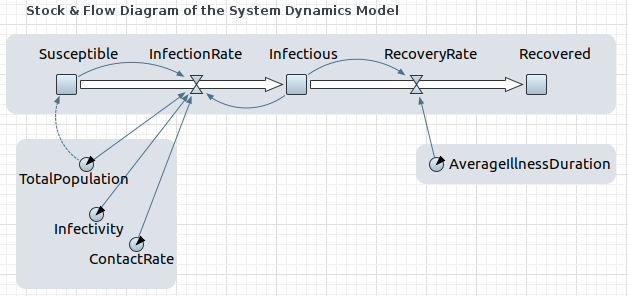
\includegraphics[width=.5\textwidth, angle=0]{./fig/SIR_SD_STOCKFLOW_DIAGRAMM.png}
	\caption{Visual System Dynamics Diagram of the SIR model in AnyLogic Personal Learning Edition 8.3.1.}
	\label{fig:sir_stockflow_diagram}
\end{figure}

Still, implementing System Dynamics directly in code is not as straight forward and involves numerical integration which can be quite tricky to get right. Thus, the aim of this paper is to look into how System Dynamics models can be implemented in code correctly without the use of a simulation package. We use the well known SIR model \cite{kermack_contribution_1927} from epidemiology to demonstrate our approach.

Our language of choice is Haskell because it emphasises a declarative programming style in which one describes \textit{what} instead of \textit{how} to compute. Further it allows to rule out interference with non-deterministic influences or side-effects already at compile-time. This is of fundamental importance for System Dynamics because it behaves completely deterministic and involves no stochastics or non-determinism whatsoever. Also, we make use of Functional Reactive Programming which allows to express continuous-time systems in a functional way. 

We show that by this approach we can arrive at correct-by-construction implementations of System Dynamic models. This means that the correctness of the code is obvious because we have closed the gap between the model specification and its implementation. Thus, the contribution of the paper is the demonstration of how to implement correct-by-construction System Dynamics simulations using Haskell and Functional Reactive Programming.

\section{Defining Agent-Based Simulation}
Agent-Based Simulation (ABS) is a methodology to model and simulate a system where the global behaviour may be unknown but the behaviour and interactions of the parts making up the system is of knowledge. Those parts, called agents, are modelled and simulated out of which then the aggregate global behaviour of the whole system emerges. So the central aspect of ABS is the concept of an agent which can be understood as a metaphor for a pro-active unit, situated in an environment, able to spawn new agents and interacting with other agents in some neighbourhood by exchange of messages \cite{wooldridge_introduction_2009}. We informally assume the following about our agents:

\begin{itemize}
	\item They are uniquely addressable entities with some internal state over which they have full, exclusive control.
	\item They are pro-active which means they can initiate actions on their own e.g. change their internal state, send messages, create new agents, terminate themselves.
	\item They are situated in an environment and can interact with it.
	\item They can interact with other agents which are situated in the same environment by means of messaging.
\end{itemize} 

Epstein \cite{epstein_generative_2012} identifies ABS to be especially applicable for analysing \textit{"spatially distributed systems of heterogeneous autonomous actors with bounded information and computing capacity"}. Thus in the line of the simulation types \textit{Statistic} $^\dag$, \textit{Markov} $^\ddag$, \textit{System Dynamics} $^\S$, \textit{Discrete Event} $^\mp$, ABS is the most powerful one as it allows to model  the following:

\begin{itemize}
	\item Linearity \& Non-Linearity $^{\dag \ddag \S \mp}$ - the dynamics of the simulation can exhibit both linear and non-linear behaviour. 
	\item Time $^{\dag \ddag \S \mp}$ - agents act over time, time is also the source of pro-activity.
	\item States $^{\ddag \S \mp}$ - agents encapsulate some state which can be accessed and changed during the simulation.
	\item Feedback-Loops $^{\S \mp}$ - because agents act continuously and their actions influence each other and themselves, feedback-loops are the norm in ABS. 
	\item Heterogeneity $^{\mp}$ - although agents can have same properties like height, sex,... the actual values can vary arbitrarily between agents.
	\item Interactions - agents can be modelled after interactions with an environment or other agents, making this a unique feature of ABS, not possible in the other simulation models.
	\item Spatiality \& Networks - agents can be situated within e.g. a spatial (discrete 2d, continuous 3d,...) or network environment, making this also a unique feature of ABS, not possible in the other simulation models.
\end{itemize}

\section{The SIR Model}
To explain the concepts of ABS and of our functional reactive approach to it, we introduce the SIR model as a motivating example. The SIR model is a a very well studied and understood compartment model from epidemiology which allows to simulate the dynamics of an infectious disease spreading through a population. In this model, people in a population of size $N$ can be in either one of three states \textit{Susceptible}, \textit{Infected} or \textit{Recovered} at a particular time, where it is assumed that initially there is at least one infected person in the population. People interact with each other \textit{on average} with a given rate $\beta$ per time-unit and get infected with a given probability $\gamma$ when interacting with an infected person. When infected, a person recovers \textit{on average} after $\delta$ time-units and is then immune to further infections. An infected person interaction with another infected one is never re-infected, thus interactions amongst infected people is not important in this model. This definition gives rise to three compartments with the transitions as seen in Figure \ref{fig:sir_transitions}.

\begin{figure}
	\centering
	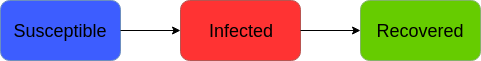
\includegraphics[width=.4\textwidth, angle=0]{./fig/SIR_transitions.png}
	\caption{Transitions in the SIR compartment model.}
	\label{fig:sir_transitions}
\end{figure}

The dynamics of this model over time can be formalized using the following equations:

$\frac{\mathrm d S}{\mathrm d t} = -infectionRate$ \\
$\frac{\mathrm d I}{\mathrm d t} = infectionRate - recoveryRate$ \\
$\frac{\mathrm d R}{\mathrm d t} = recoveryRate$ \\

$infectionRate = \frac{I \beta S \gamma}{N}$ \\
$recoveryRate = \frac{I}{\delta}$ \\

Solving these can be done using the System-Dynamics (SD) approach which solves the equations by integrating over time. In the SD terminology, the intergrals are called \textit{Stocks} and the values over which is integrated over time are called \textit{Flows}.

$S(t) = N + \int_0^t -infectionRate\, \mathrm{d}t$ \\
$I(t) = 1 + \int_0^t infectionRate - recoveryRate\, \mathrm{d}t$ \\
$R(t) = \int_0^t recoveryRate\, \mathrm{d}t$ \\

There exist a huge number of software-packages which allow to conveniently express SD models using a visual approach like in Figure \ref{fig:sir_sd_stockflow_diagramm}.

\begin{figure}
	\centering
	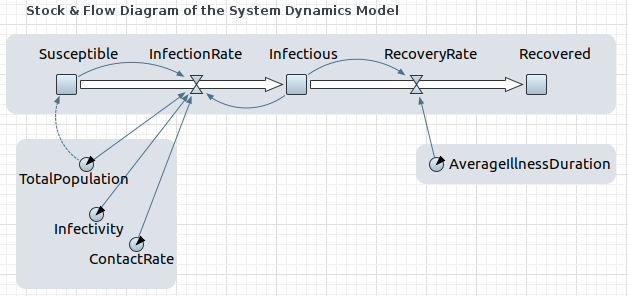
\includegraphics[width=.4\textwidth, angle=0]{./fig/SIR_SD_STOCKFLOW_DIAGRAMM.png}
	\caption{A visual representation of the stocks and flows in the SIR compartment model (Image courtesy of AnyLogic Company).}
	\label{fig:sir_sd_stockflow_diagramm}
\end{figure}

Running the SD simulation over time results in the dynamics as shown in Figure \ref{fig:sir_sd_dynamics_anylogic} with the given variables.

\begin{figure}
	\centering
	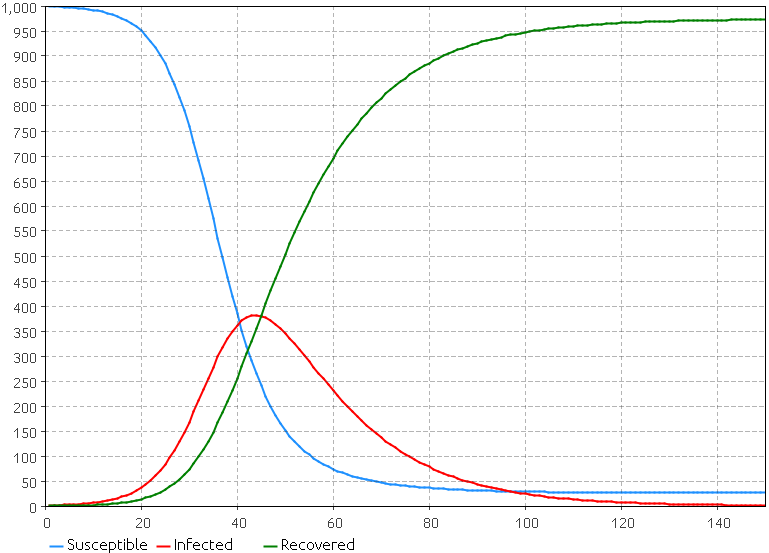
\includegraphics[width=.4\textwidth, angle=0]{./fig/SIR_SD_DYNAMICS_ANYLOGIC.png}
	\caption{Dynamics of the SIR compartment model using the System Dynamics approach generated with the AnyLogic Personal Learning Edition 8.1.0. Population Size $N$ = 1000, contact rate $\beta = 1/5$, infection probability $\gamma = 0.05$, illness duration $\delta = 15$.}
	\label{fig:sir_sd_dynamics_anylogic}
\end{figure}

\subsection{An Agent-Based approach}
The SD approach is inherently Top-Down because the emergent property of the system is formalized in differential equations. The question is if such a top-down behaviour can be emulated using ABS, which is inherently bottom-up. Also the question is if there are fundamental drawbacks and benefits when doing so using ABS. Indeed such questions were asked before and modelling the SD approach of the SIR model is possible using an agent-based approach. It is important to note that SD treats the population completely continuous which results in non-discrete values of stocks e.g. 3.1415 infected persons. Thus the fundamental approach to map the SIR model to an ABS is to discretisize the population and model each person in the population as an invidivual agent. The transition  between the states are no longer happening according to continuous differential equations but due to discrete events caused both by interactions amongst the agents and time-outs. The behaviour can be defined as follows:

\begin{itemize}
	\item Every agent makes on average contact with $\beta$ random other agents per time unit. In ABS we can only contact discrete agents thus we model this by generating a random event on average every $\beta$ time units.
	
	\item An agent does not know the other agents state when making contact with it, thus we need a mechanism in which agents reveal their state in which they are in \textit{at the moment of making contact}. Obviously the already mentioned messaging-mechanism which allows agents to interact is perfectly suited to do this.
	\begin{itemize}
		\item \textit{Susceptible} agent: sends a "Susceptible" message when contacting another agent. There is no need to reply to other incoming messages as making contact with a susceptible agent has no influence on the state of an agent.
		\item \textit{Infected} agent: sends a "Infected" message when contacting another agent. An infected agent now needs to reply to incoming "Susceptible" messages with an "Infected" message to let the susceptible agent know that it has made contact with an infected agent.
		\item \textit{Recovered} agent: does not need to send messages because contacting it or being contacted by it has no influence on the state.
	\end{itemize}
	
	\item Susceptible to Infected: needs to have made contact with an infected agent which happens when it receives an "Infected" message. If this occurs an infection occurs with a probability of $\gamma$. The infection can be calculated by drawing from a uniform random-distribution between 0 and 1 and comparing the value to $\gamma$, if the drawn value $p < \gamma$ then infection occurs. Note that this needs to be done for \textit{every} received "Infected" message.
	
	\item Infected to Recovered: a person recovers \textit{on average} after $\delta$ time unites. This is implemented by drawing the duration from an exponential distribution (TODO: borchschev) with $\lambda = \frac{1}{\delta}$ and making the transition after this duration.
\end{itemize}

We will discuss the implementation of this approach in the following sections and as will be shown FrABS will allow us to express this behaviour very explicitly looking very much like a formal ABS specification of the problem. For now we will give the resulting dynamics in Figure TODO

TODO: how many initially infected agents? one should be enough, at least in my implementation

TODO: 100 vs. 1000 vs. 5.000 agents

TODO: problem in my code: need exponentially occasionally not uniform distributed! => OK, occasionally draws from exponential-distribution
TODO: what differences do the different update strategies make?

\subsection{Blub}
TODO: It should be possible to formally show that spatial SIR and WildFire are the same model. NOTE: they are NOT the same, the fundamental difference is that in the WildFire model only the burning cells initiate the ignition - if we compare this to the SIR, the burning cells would be infected agents and although in the spatial SIR model the infected agents make contact with other agents, so do the susceptible ones which does NOT occur in wildfire

TODO: cite my own work on update-strategies

TODO: can we formally show that the SIR approximates the SD model?

TODO: cite papers which discuss how to approximate a SD model by ABS
- Macal (2010) - To Agent-Based Simulation From System Dynamics 
	-> i am very unhappy with this paper: first it does not give concrete parameters for the SD model so it is impossible to replicate. Also i think it has a systematical error as the infected agents make no contact but this is required as evident from the SD-models infection-rate which also incorporates. TODO: write an email to this guy: why are the infectious not contacting the other agents? this seems to be a systematical error
- Borshchev, Filippov (2004) - From System Dynamics and Discrete Event to Practical Agent Based Modeling: Reasons, Techniques, Tools
	-> its VERY IMPORTANT point is that we need to draw the illness-duration from an exponential-distribution because the illness-duration is proportional to the size of the infected. note: this is wrongly expressed, need to find the correct formulation

		-> my emulation of SD using ABS is really an implementation of the SD model and follows it - they are equivalent
		-> my ABS implementation is the same as / equivalent to the SD emulation
			=> thus if i can show that my SD emulation is equlas to the SD model
			=> AND that the ABS implementation is the same as the SD emulation
			=> THEN the ABS implementation is an SD implementation, and we have shown this in code for the first time in ABS
			


\section{Functional Reactive ABS}
%TODO: cross reference to the code in the appendix by giving line-numbers e.g. the full implementation of a susceptible agent can be seen in

The challenges one faces when implementing an ABS plain, without support from a library are manifold. Generally one faces the following challenges:

\begin{itemize}
	\item Agent Representation - how do we represent an agent in Haskell?
	\item Agent-Agent Interaction - how can agents interact with other agents in Haskell without resorting to the IO Monad?
	\item Environment representation - how can we represent an environment which must have the ability to update itself e.g. regrow some resources?
	\item Agent-Environment interaction - how can agents interact (read / write) with the environment?
	\item Agent Updating - how is the set of agents organised, how are they updated and how is it managed (deleting, adding during simulation) in Haskell without resorting to the IO Monad?
\end{itemize}

In the next subsections we will discuss each point by deriving a functional reactive implementation of the agent-based SIR model. For us it is absolutely paramount that the simulation should be pure and never run in the IO Monad (except of course the surrounding Yampa loop which allows rendering and output). The complete source-code can be seen in Appendix \ref{app:abs_code}.

\subsection{Agent Representation}
An agent can be seen as a tuple $<id, s, m, e, b>$.
\begin{itemize}
	\item \textbf{id} - the unique identifier of the agent
	\item \textbf{s} - the generic state of the agent
	\item \textbf{m} - the messages the agent understands
	\item \textbf{e} - the environment the agent can interact with
	\item \textbf{b} - the behaviour of the agent
\end{itemize}

The id is simply represented as an Integer and must be unique for all currently existing agents in the system as it is used for message delivery. %A stronger requirement would be that the id of an agent is unique for the whole simulation-run and will never be reused - this would support replications and operations requiring unique agent-ids.

Each agent may have a generic state which could be represented by any data type or compound data. A SIR agent's state can be represented using the an Algebraic Data Type (ADT) as follows:
\begin{minted}[fontsize=\footnotesize]{haskell}
data SIRState = Susceptible | Infected | Recovered
\end{minted}

The behaviour of the agent is a signal-function which maps a tuple of an AgentIn and the environment to an AgentOut and the environment. It has the following signature \footnote{Note that we omit the type-parameters in the following code-listings unless it is needed for clarity. Still it is important to keep in mind that all AgentIn and AgentOut are parameterised with \textit{s} representing the type of its state, \textit{m} representing the type of the messages and \textit{e} representing the type of environment.} 
\begin{minted}[fontsize=\footnotesize]{haskell}
type AgentBehaviour s m e = SF (AgentIn s m e, e) (AgentOut s m e, e)
\end{minted}

\textit{AgentIn} provides the necessary data to the agent-behaviour: its \textit{id}, incoming messages, the current state \textit{s} and a random-number generator. \textit{AgentOut} allows the agent to communicate changes: kill itself, create new agents, sending messages, an updated state \textit{s} and a changed random-number generator. Both types are opaque and access to them is only possible through the provided functions. The behaviour also gets the environment passed in, which the agent can read and also write by changing it and returning it along side the \textit{AgentOut}. It is important to note that the environment is completely generic and we do not induce any type bounds on it. Obviously \textit{AgentIn} is read-only whereas \textit{AgentOut} is both read- and write-able. The first thing an agent-behaviour does is creating the default AgentOut from the existing AgentIn as is done in line 94 in Appendix \ref{app:abs_code}.

\begin{minted}[fontsize=\footnotesize]{haskell}
agentOutFromIn :: AgentIn -> AgentOut
\end{minted}

This will copy the relevant fields over to \textit{AgentOut} on which one now primarily acts. The read-only and read/write character of both types is also reflected in the EDSL where most of the functions implemented also work that way: they may read the \textit{AgentIn} and read/write an \textit{AgentOut}. Relevant functions for working on the agent-definition are:

\begin{minted}[fontsize=\footnotesize]{haskell}
type AgentId = Int

agentId :: AgentIn -> AgentId
kill :: AgentOut -> AgentOut
isDead :: AgentOut -> Bool
onStart :: (AgentOut -> AgentOut) -> AgentIn -> AgentOut -> AgentOut

agentState :: AgentOut -> s
setAgentState :: s -> AgentOut -> AgentOut
updateAgentState :: (s -> s) -> AgentOut -> AgentOut

createAgent :: AgentDef -> AgentOut -> AgentOut
\end{minted}

The function \textit{kill} marks an agent for removal after the current iteration. The function \textit{isDead} checks if the agent is marked for removal. The function \textit{onStart} allows to change the \textit{AgentOut} in the case of the start-event which happens on the very first time the agent runs. The function \textit{agentState} returns the agents' state \textit{s}, \textit{setAgentState} allows to change the state of the agent by overriding it and \textit{updateAgentState} allows to change it by keeping parts of it. The function \textit{createAgent} allows to add an agent-definition \footnote{AgentDef simply contains the initial state, behaviour and id of the agent (amongst others). See line 50 - 57 in Appendix \ref{app:abs_code}.} to the AgentOut which results in creating a new agent from the given definition which will be active in the next iteration of the simulation. 

Having these functions we build some reactive primitives into our EDSL meaning that they return signal-functions themselves. We start with the following functions:

\begin{minted}[fontsize=\footnotesize]{haskell}
doOnce :: (AgentOut -> AgentOut) -> SF AgentOut AgentOut
doOnceR :: AgentBehaviour -> AgentBehaviour
doNothing :: AgentBehaviour

setAgentStateR :: s -> AgentBehaviour
updateAgentStateR :: (s -> s) -> AgentBehaviour
\end{minted}

The \textit{doOnce} function may seem strange at first but allows conveniently make actions (which are changing the \textit{AgentOut}) only once e.g. when making the transition from Susceptible to Infected changing the state to Infected just once as can be seen in line 114 of Appendix \ref{app:abs_code}. A more striking example would be to send a message just once after a transition. The \textit{doOnceR} function is the reactive version, which allows to run an agent behaviour only once. The function \textit{doNothing} provides a convenient way of an agent sink which is basically an agent which does literally nothing - the resulting agent behaviour just transforms the \textit{AgentIn} to \textit{AgentOut} using the previously mentioned function \textit{agentOutFromIn}.

Often we want some more reactive behaviour e.g. making a transition from one behaviour to another on a given event. For this we provide the following:

\begin{minted}[fontsize=\footnotesize]{haskell}
type EventSource = SF (AgentIn, AgentOut) (AgentOut, Event ())
transitionOnEvent :: EventSource -> AgentBehaviour -> AgentBehaviour -> AgentBehaviour
\end{minted}

The function \textit{transitionOnEvent} takes an event-source which creates the event, an agent behaviour which is run until the event hits and an agent behaviour which is run at the event and after. The event-source is a signal-function itself to allow maximum of flexibility and gets both \textit{AgentIn} and \textit{AgentOut} and returns a (potentially changed) \textit{AgentOut} and the event upon to switch. 
This function is used for implementing the susceptible agent where we use a \textit{transitionOnEvent} and a specific event-source which generates an event when the susceptible agent got infected as can be seen in lines 81-90 in Appendix \ref{app:abs_code}.

Sometimes we need our transition event to rely on time-semantics e.g. in SIR where an infected agent recovers \textit{on average} after $\delta$ time-units. For this we provide the following function which can be seen in line 106 in Appendix \ref{app:abs_code}:

\begin{minted}[fontsize=\footnotesize]{haskell}
transitionAfterExp :: RandomGen g => g -> Double -> AgentBehaviour -> AgentBehaviour -> AgentBehaviour
\end{minted}

It takes a random-number generator, the \textit{average} time-out, the behaviour to run before the time-out and the behaviour to run after the time-out where the function will return then the according behaviour. For implementing this behaviour we initially used Yampas \textit{after} function which generates an event after given time-units but this would not result in the correct dynamics as we rather need to create a random-distribution of time-outs than a deterministic time-out which occurs always after the same time. For this we implemented our own function, called \textit{afterExp}, which now takes a random-number generator a time-out and some value of type b and creates a signal-function which ignores its input and creates an event \textit{on average} after DTime.

\begin{minted}[fontsize=\footnotesize]{haskell}
afterExp :: RandomGen g => g -> DTime -> b -> SF a (Event b)
\end{minted}

\subsection{Agent-Agent Interaction}
Agent-agent interaction is the means of an agent to directly address another agent and vice versa. Inspired by the actor model we implement  \textit{messaging} with share-nothing semantics. In this case the agent sends messages which will arrive at the receiver in the next step of the simulation, thus being kind of asynchronous - a round-trip would always take at least two steps, independent of the sampling time. Depending on the semantics of the model we sometimes need synchronous interactions e.g. when only one agent can change the environment or decisions need to be made within one step - this wouldn't be possible with the asynchronous messaging. For this we introduced the concept of \textit{conversations} which allow two agents to interact with each other for an arbitrary number of requests and replies without the simulation being advanced - time is halted and only the two agents are active until they finish their conversation.

\subsubsection{Messaging}
Each Agent can send a message to another agent through \textit{AgentOut} where incoming messages are queued in the \textit{AgentIn} in unspecified order and can be processed when the agent is running the next time. The agent is free to ignore the messages and if it does not process them in the current step, they will simply be lost. This is in fundamental contrast to the actor model where messages stay in the message-box of the receiving actor until the actor has processed them. We chose a different approach as time has a different meaning in ABS than in a system of actors where there is basically no global notion of time.
Note that due to the fact we don't have method-calls in FP, messaging will always take some time, which depends on the sampling interval of the system. This was not obviously clear when implementing ABS in an object-oriented way because there we can communicate through method calls which are a way of interaction which takes no simulation-time.
For messaging, we need a set of messages \textit{m} the agents understand. In the case of the SIR model we simply use the following:

\begin{minted}[fontsize=\footnotesize]{haskell}
data SIRMsg = Contact SIRState
\end{minted}

In addition we provide the following functions in our EDSL to support messaging.

\begin{minted}[fontsize=\footnotesize]{haskell}
type AgentMessage m = (AgentId, m)

sendMessage :: AgentMessage m -> AgentOut -> AgentOut
sendMessageTo :: AgentId -> m -> AgentOut -> AgentOut
sendMessages :: [AgentMessage m] -> AgentOut -> AgentOut
broadcastMessage :: m -> [AgentId] -> AgentOut -> AgentOut

hasMessage :: (Eq m) => m -> AgentIn -> Bool
onMessage :: (AgentMessage -> acc -> acc) -> AgentIn -> acc -> acc
onMessageFrom :: AgentId -> (AgentMessage -> acc -> acc) -> AgentIn -> acc -> acc
onMessageType :: (Eq m) => m -> (AgentMessage -> acc -> acc) -> AgentIn -> acc -> acc
\end{minted}

Most of the functions are pretty self-explanatory, we will shortly explain the \textit{onMessage*}. The function \textit{onMessage} provides a way to react to incoming messages by using a callback function which manipulates an accumulator, thus resembling the workings of fold. The functions \textit{onMessageFrom} and \textit{onMessageType} provide the same functionality but filter the messages accordingly. We can now write implement the functionality of an infected agent which replies to an incoming \textit{Contact} message with another \textit{Contact Infected} message as can be seen in line 73 of Appendix \ref{app:abs_code}.

Sometimes we also need discrete semantics like changing the behaviour of an agent on reception of a specific message. For this we provide the function \textit{transitionOnMessage} which works the same way as \textit{transitionOnEvent} but now on a message instead.

\begin{minted}[fontsize=\footnotesize]{haskell}
transitionOnMessage :: (Eq m) => m -> AgentBehaviour -> AgentBehaviour -> AgentBehaviour
\end{minted}

Of course messaging sometimes may have specific time-semantics as in our SIR model. There susceptible agents make contact with $\beta$ other agents on average \textit{per time unit}. To implement this we randomly need to generate messages with a given frequency within some time-interval by drawing from the exponential random-distribution. This is already supported by Yampa using \textit{occasionally} and we have built on it a the following:

\begin{minted}[fontsize=\footnotesize]{haskell}
type MessageSource m e = e -> AgentOut -> (AgentOut, AgentMessage m)

sendMessageOccasionallySrc :: RandomGen g => g -> Double -> MessageSource -> SF (AgentOut, e) AgentOut

constMsgReceiverSource :: m -> AgentId -> MessageSource 
randomNeighbourNodeMsgSource :: m -> MessageSource s m (Network l)
randomNeighbourCellMsgSource :: (s -> Discrete2dCoord) -> m -> Bool -> MessageSource s m (Discrete2d AgentId)
randomAgentIdMsgSource :: m -> Bool -> MessageSource s m [AgentId]
\end{minted}

The function \textit{sendMessageOccasionallySrc} takes a random-number generator, the frequency of messages to generate \textit{on average per time-unit} a message-source and returns a signal-function which takes a tuple of an \textit{AgentOut} and environment and returns an \textit{AgentOut}. This signal-function which performs the actual generating of the messages needs to be fed in the tuple but only returns the changed \textit{AgentOut} but not the environment - this guarantees statically at compile-time that the environment cannot be changed in this process. This is also directly reflected in the type of \textit{MessageSource} which takes an environment and \textit{AgentOut} and returns a tuple with a changed \textit{AgentOut} and a message. We provide pre-defined messages-sources like \textit{constMsgReceiverSource} which always generates the same message, \textit{randomNeighbourNodeMsgSource} which picks a random neighbour from a network-environment (see below), \textit{randomNeighbourCellMsgSource} which picks a random neighbour from a discrete 2D grid environment (see below) and \textit{randomAgentIdMsgSource} which randomly picks an element from an environment which is a list of \textit{AgentId} (omitting the sender True/False). The susceptible agent builds on this function to make contact with other agents as can be seen in line 96-100 of Appendix \ref{app:abs_code}.

\subsubsection{Conversations}
The messaging as implemented above works well for one-directional, virtual asynchronous interaction where we don't need a reply at the same time. A perfect use-case for messaging is making contact with neighbours in the SIRS-model: the agent sends the contact message but does not need any response from the receiver, the receiver handles the message and may get infected but does not need to communicate this back to the sender. 
A different case is when agents need to transact in the same time-step or interact over multiple steps: agent A interacts with agent B where the semantics of the model need an immediate response from agent B - which can lead to further interactions initiated by agent A. An example would be negotiating a trading price between two agents to buy and sell goods between each other and then execute the trade. This must happen in the same time-step as constraints need to be considered which could be violated in asynchronous interactions. Basically the concept is always the same and is rooted in the fact that these interactions needs to transact in the current time-step as all of the actions only work on a 1:1 relationship and could violate resource-constraints.
For this we introduce the concept of a \textit{conversation} between agents. It allows an agent A to initiate a conversation with another agent B in which the simulation is virtually halted and both can exchange an arbitrary number of messages through calling and responding without time passing, something not possible without this concept because in each iteration the time advances. After either one agent has finished with the conversation it will terminate it and the simulation will continue with the updated agents. It is important to understand that \textit{both} agents can change their state and the envirionment in a conversation. The conversation concept is implemented at the moment in the way that the initiating agent A has all the freedom in sending messages, starting a new conversation,... but that the receiving agent B is only able to change its state but is not allowed to send messages or start conversations in this process. Technically speaking: agent A can manipulate an \textit{AgentOut} whereas agent B can only read its \textit{AgentIn} and manipulate its state.
When looking at conversations they may look like an emulation of method-calls but they are more powerful: a receiver can be unavailable to conversations or simply refuse to handle this conversation. This follows the concept of an active actor which can decide what happens with the incoming interaction-request, instead of the passive object which cannot decide whether the method-call is really executed or not.

\begin{minted}[fontsize=\footnotesize]{haskell}
type AgentConversationReceiver s m e = AgentIn -> e -> AgentMessage m -> Maybe (s, m, e)
type AgentConversationSender m e = AgentOut -> e -> Maybe (AgentMessage m) -> (AgentOute, e)
                                        
conversation :: AgentMessage m -> AgentConversationSender -> AgentOut -> AgentOut
conversationEnd :: AgentOut -> AgentOut 
\end{minted}

The conversation sender is the initiator of the conversation which can only be an agent which is just run and has started a conversation with a call to the function \textit{conversation}. After the agent has run, the simulation system will detect the request for a conversation and start processing it by looking up the receiver and calling the functions with passing the values back and forth. While a conversation is active, time does not advance and other agents do not act. Note that due to its nature, conversations are only available when using the \textit{sequential} update-strategy (see below). Note that conversations are inherently non-reactive because they are synchronous interactions, involve no time-semantics because time is halted, thus it makes no sense to implement conversations as signal-functions.

\subsection{Environment representation}
Agents have access to an environment which itself is \textit{not} an agent - although it can have its own behaviour e.g. regrowing resources, it cannot send or receive messages from agents. Thus we treat the environment completely generic by allowing any given type captured in the type-variable \textit{e}. Environment behaviour is optional but if required, implemented using a signal-function which simply maps \textit{e} to \textit{e}:

\begin{minted}[fontsize=\footnotesize]{haskell}
type EnvironmentBehaviour e = SF e e
\end{minted}

By allowing a signal-function as the environment behaviour gives us the opportunity to implement reactive behaviour and time-semantics in environments as well. Again it is essential to note that throughout the whole simulation implementation we never put any bounds on the environment nor make assumptions about its type \footnote{Exceptions in case when providing utility-functions which allow agents to operate on existing environment implementations}.

Although environments can be anything, even be of unit-type \textit{()} if no environment is required at all, there exist a few standard environments in ABS which are provided in all ABS packages. We provide implementations for them and discuss them below. Note that we don't provide the APIs of the environments here as it is out of the scope of this paper.

\subsubsection{Network}
A network environment gives agents access to a network, represented by a graph where the nodes are agent-ids and the edges represent neighbourhood information. We implemented fully-connected, Erdos-Renyi and Barbasi-Albert networks. In our case the networks are undirected and the labels can be labelled, carrying arbitrary data or being unlabelled, having unit-type. Agents can then perform the usual graph algorithms on these networks. 

\subsubsection{Discrete 2D}
A discrete 2d environment gives agents access to a 2D grid with dimensions of $N \times M \in \mathbb{N}$ cells. The cells are of a generic type $c$ and can thus be anything from \textit{AgentId} to resource-sites with single or multiple occupants. Such an environment has a defined neighbourhood of either Moore (8 neighbours) or Von-Neumann (4 neighbours). Agents can then query the environment for cells using neighbourhoods, radius or specific positions, change the cells and update them in the environment.

\subsubsection{Continuous 2D}
A continuous 2d environment gives agents access to a continuous 2D space with dimensions of $N \times M \in \mathbb{R}$. This space can contain an arbitrary number of objects of the generic type \textit{o} where each of them has a coordinate within this space. Agents can query for objects within a given radius, add, remove and update them. Also we provide functions to move objects either in a given or random direction.

\subsection{Agent-Environment interaction}
In ABS agents almost always are \textit{situated within} an environment. We follow a subtle different approach and implement it in a way that agents have access to a generic environment of type $e$ as discussed above instead of being situated within. It is important to note the subtle difference of agents having \textit{access to} the environments instead of \textit{being situated} within them. This allows to free us making assumptions within an environment how agents use these environments and also allows us to stack multiple environments e.g. agents moving on a discrete 2D grid but relying on neighbourhood from a network.
Our SIR implementation uses a list of all \textit{AgentId} as the environment which means that every agent knows all the existing agents of the simulation and can address them - see line 6 in \ref{app:abs_code}. We could have used a Network environment using a fully-connected graph but the memory-consumptions of the library \textit{FGL} we are using for graphs are unacceptable in case of fully-connected networks of a larger numbers of agents (10,000). Each agent gets the environment passed in through the \textit{AgentIn} and can change it by passing a changed version of the environment out through \textit{AgentOut}. 

\subsection{Agent Updating}
For agents to be pro-active, they need to be able to perceive time. Also agents must have the opportunity to react to incoming messages and manipulate the environment. The work of (TODO: cite our own paper on update-strategies) identifies four possible ways of doing this where we only implemented the \textit{sequential-} and \textit{parallel-strategy} \footnote{The other two strategies being the  \textit{concurrent-} and \textit{actor-strategy}, both requiring to run within the STM-Monad, which is not possible with Yampa. Ivan Perez \cite{perez_functional_2016} implemented a library called \textit{Dunai}, which is the same as Yampa but capable of running in an arbitrary Monad. We leave this for further research.}. Implementing these iteration-strategies using Haskell and FRP is not as straight-forward as in imperative effectful languages because one does not have mutable data which can be updated in-place. 
We implement both update-strategies basically by running all agents behaviour signal-functions every $\Delta t$, so when running a simulation for a duration of \textit{t} the number of steps is $\frac{t}{\Delta t}$. It is important to realise that in our approach of a single behaviour function we merge pro-activity, time-dependent behaviour and message receiving behaviour. A different approach would be to have callbacks for messages in addition to the normal agent-behaviour but this would be quite cluttered and inelegant.

In both the sequential and parallel update-strategy each iteration must also output a potentially changed environment. As already discussed this is implemented as a signal-function which, when available, is then run after each iteration, to make the environment pro-active as well. An example of an environment behaviour would be to regrow some good on each cell according to some rate per time-unit.

\subsubsection{Sequential}
In this strategy the agents are updated one after another where the changes (messages sent, environment changed,...) of one agent are visible to agents updated after. Basically this strategy is implemented as a variant of \textit{fold} which allows to feed output of one agent (e.g. messages and the environment) forward to the other agents while iterating over the list of agents. For each agent the agent behaviour signal-function is called with the current \textit{AgentIn} as input to retrieve the according \textit{AgentOut}. The messages of the \textit{AgentOut} are then distributed to the \textit{AgentIn} of the receiving agents.
The environment which is passed in and returned as well, will then be passed forward to the next agent$_{i + 1}$ in the current iteration. The last environment is then the final environment in the current iteration and will be returned together with the current list of \textit{AgentOut} (see below). As previously mentioned, conversations are \textit{only} possible within this update-strategy because only in this strategy agents act after another which is a fundamental requirement for conversations to make sense and work correctly.

\subsubsection{Parallel}
The parallel strategy is \textit{much} easier to implement than the sequential but is of course not applicable to all models because of its different semantics. Basically this strategy is implemented as a \textit{map} over all agents which calls each agent behaviour signal-function with the agents \textit{AgentIn} to retrieve the new \textit{AgentOut}. Then the messages are distributed amongst all agents.
Each agent receives a copy of the environment upon which it can work and return a changed one. Thus after one iteration there are \textit{N} versions of environments where \textit{N} is equals to the number of agents. These environments must then be folded into a final one which is always domain-specific thus the model implementer needs to provide a corresponding function.

\begin{minted}[fontsize=\footnotesize]{haskell}
type EnvironmentFolding e = [e] -> e
\end{minted}

Of course not all models have environments which can be changed and in the SIR model we indeed use a list of AgentIds which won't change during execution, meaning the agents only read it. Because of this, the environment folding function is optional and when none is provided the environments returned by the agents are ignored and always the initial one is provided.
To make this more explicit we introduce a wrapper which wraps a signal-function which is the same as agent-behaviour but omits the environment from the out tuples. When this wrapper is used one can guarantee statically at compile-time that the environment cannot be changed by the agent-behaviour. We also provide a function which completely ignores the environment, which allows to reason already at compile time that no environment access will happen ever in the given signal-function.

\begin{minted}[fontsize=\footnotesize]{haskell}
type ReactiveBehaviourIgnoreEnv = SF AgentIn AgentOut
type ReactiveBehaviourReadEnv e = SF (AgentIn, e) AgentOut

ignoreEnv :: ReactiveBehaviourIgnoreEnv -> AgentBehaviour
readEnv :: ReactiveBehaviourReadEnv -> AgentBehaviour
\end{minted}

We use both functions in our SIR implementation. The function \textit{readEnv} is used in line 83 of Appendix \ref{app:abs_code} to make sure the behaviour of a susceptible agent can read the environment but never change it. The function \textit{ignoreEnv} is used in line 110 of Appendix \ref{app:abs_code} to make sure the behaviour of an infected agent never accesses the environment.

\subsection{Non-Reactive Features}
Not all models have such explicit time-semantics as the SIR model. Such models just assume that the agents act in some order but don't rely on any time-outs, timed transitions or rates. These models are more of an imperative nature and map therefore naturally to a monadic style of programming using the \textit{do} notation. Unfortunately it is not possible to do monadic programming within a signal-function, thus to support the programming of such imperative models, we implemented wrapper-functions which allow to provide both non-monadic and monadic functionality which runs within a wrapper signal-function.

\subsubsection{Non-monadic (pure) wrapping}

\begin{minted}[fontsize=\footnotesize]{haskell}
agentPure :: (e -> Double -> AgentIn -> AgentOut -> (AgentOut, e)) -> AgentBehaviour
agentPureReadEnv :: (e -> Double -> AgentIn -> AgentOut -> AgentOut) -> AgentBehaviour
agentPureIgnoreEnv :: (Double -> AgentIn -> AgentOut -> AgentOut) -> AgentBehaviour
\end{minted}

The function \textit{agentPure} wraps a non-monadic (pure) function and wraps it in a signal-function. This pure function has the environment, the current local time of the agent, the \textit{AgentIn} and a default \textit{AgentOut} as arguments and must return the tuple of \textit{AgentOut} and the environment.
The function \textit{agentPureReadEnv} works the same as \textit{agentPure} but omits the environment from the return type thus ensuring statically at compile-time that an agent which implements its behaviour in this way can only read the environment but never change it.
The function \textit{agentPureIgnoreEnv} is an even more restrictive version and omits environment from the agents behaviour altogether thus ensuring statically at compile-time that an agent which wraps its behaviour in this function will never access the environment.

\subsubsection{Monadic wrapping}
The monadic wrappers work basically the same way as the pure version, with the difference that they run within the state-monad with \textit{AgentOut} being the state to pass around.

\begin{minted}[fontsize=\footnotesize]{haskell}
agentMonadic :: (e -> Double -> AgentIn -> State AgentOut e) -> AgentBehaviour
agentMonadicReadEnv :: (e -> Double -> AgentIn -> State AgentOut ()) -> AgentBehaviour
agentMonadicIgnoreEnv :: (Double -> AgentIn -> State AgentOut ()) -> AgentBehaviour
\end{minted}

We also provide monadic versions of the pure primitives of our EDSL which work on \textit{AgentOut} as discussed above. They run in the State Monad where the state is the \textit{AgentOut} as this is the data which is manipulated step-by-step for the final output. 

\begin{minted}[fontsize=\footnotesize]{haskell}
agentIdM :: State (AgentOut s m e) AgentId

sendMessageM :: AgentMessage m -> State AgentOut ()
sendMessageToM :: AgentId -> m -> State AgentOut ()
onMessageM :: (Monad mon) => (acc -> AgentMessage m -> mon acc) -> AgentIn -> acc -> mon acc

createAgentM :: AgentDef -> State AgentOut ()

killM :: State AgentOut ()
isDeadM :: State AgentOut Bool

agentStateM :: State AgentOut s
updateAgentStateM :: (s -> s) -> State AgentOut ()
setAgentStateM :: s -> State AgentOut ()
agentStateFieldM :: (s -> t) -> State AgentOut t
\end{minted}

For the environment-behaviour we provide a monadic wrapper as well.

\begin{minted}[fontsize=\footnotesize]{haskell}
type EnvironmentMonadicBehaviour e = Double -> State e ()
environmentMonadic :: EnvironmentMonadicBehaviour e -> EnvironmentBehaviour e
\end{minted}

\subsection{Randomness}
Most of the ABS are inherent stochastic processes and so is the agent-based SIR implementation. This means that agents behaviour depends on random-numbers. So far the drawing from these random-number was hidden behind functions but sometimes an agent needs to draw a random-number directly. For this we provide each agent with its own random-number generator which must be initialized when creating the agent-definition as seen in line 48-59 of Appendix \ref{app:abs_code}. The agent can then draw random-numbers in a pure way without having to resort to the IO Monad. Still it can become very cumbersome because the changed random-number generator needs to be updated in the opaque \textit{AgentOut} - for this we provide a few convenience functions and monadic implementations.

\begin{minted}[fontsize=\footnotesize]{haskell}
agentRandom :: Rand StdGen a -> AgentOut -> (a, AgentOut)
agentRandomM :: Rand StdGen a -> State AgentOut a

randomBoolM :: (RandomGen g) => Double -> Rand g Bool
\end{minted}

Both functions \textit{agentRandom} and \textit{agentRandomM} allow to run a random action implemented in the Rand Monad acting on a StdGen generator. Both need an instance of an \textit{AgentOut} which runs the random action on the agents random-number generator, updates it and returns the random value.
The function \textit{randomBoolM} is such a random action implemented in the Rand Monad and draws a random boolean which is True with a given probability. It is use to randomly determine if a susceptible agent got infected in case of a \textit{Contact Infected} message as can be seen in line 67 of Appendix \ref{app:abs_code}. Note that this random action runs in \textit{onMessageM} which allows to run on a generic monad. Note there exist more random action e.g. to pick at random from a list, to randomly generate within a range, to shuffle a list and to draw from a random distribution. We didn't discuss them here as they follow the same principle.

\subsection{Running the Simulation}
For actually running the simulation we provide three different approaches. 

\begin{minted}[fontsize=\footnotesize]{haskell}
type AgentObservable s = (AgentId, s)
type SimulationStepOut s e = (Time, [AgentObservable s], e)
type AgentObservableAggregator s e a = SimulationStepOut s e -> a

simulateIOInit :: [AgentDef] -> e -> SimulationParams e
                    -> (ReactHandle () (SimulationStepOut s e) -> Bool -> SimulationStepOut s e -> IO Bool)
                    -> IO (ReactHandle () (SimulationStepOut s e))
                    
simulateTime :: [AgentDef] -> e -> SimulationParams e -> DTime -> Time -> [SimulationStepOut s e]
simulateAggregateTime :: [AgentDef] -> e -> SimulationParams -> DTime -> Time -> AgentObservableAggregator a -> [a]
simulateTimeDeltas :: [AgentDef] -> e -> SimulationParams e -> [DTime] -> [SimulationStepOut s e]
\end{minted}

The first one \textit{simulateIOInit} allows for output in the IO Monad, which is useful when one wants to run the simulation for an undefined number of steps and visualise each step by rendering it to a window using a rendering library e.g. \textit{Gloss} \footnote{Note that we provide substantial rendering functionality for the environments but don't discuss it here as it is out of the scope of the paper.}. The \textit{ReactHandle} is part of Yampas function \textit{reactinit} and we refer to Yampas documentation for further details. The second approach \textit{simulateTime} runs the simulation for a given time with given $\Delta t$ and then returns the output for all $\Delta t$. The third approach \textit{simulateTimeDeltas} works the same as the second one but one can provide a list of all $\Delta t$. The function \textit{simulateAggregateTime} allows to transform the output of each step into a different representation, as happens in our SIR implementation where we aggregate the list of all observable agent-outputs into a tuple holding the number of susceptible, infected an recovered agents (see line 136 and 139 - 144 of Appendix \ref{app:abs_code}).
In all approaches at every $\Delta t$ we output a tuple of the current global simulation time, a list of \textit{AgentId} with their states \textit{s} and the environment \textit{e}. All approaches take a list of initial agent definitions, the initial environment and simulation parameters which are obtained calling the function \textit{initSimulation}:

\begin{minted}[fontsize=\footnotesize]{haskell}
data UpdateStrategy = Sequential | Parallel deriving (Eq)

initSimulation :: UpdateStrategy
                    -> Maybe (EnvironmentBehaviour e)
                    -> Maybe (EnvironmentFolding e)
                    -> Bool
                    -> Maybe Int
                    -> IO (SimulationParams e)
\end{minted}

This function takes as parameters the update-strategy with which to run this simulation, an optional environment behaviour, an optional environment folding, a boolean which determines whether the agents are shuffled after each iteration \footnote{This is necessary in some models which run in the sequential strategy to uniformly distribute the probability of an agent to run at a fixed position.} and an optional initial random-number generator seed.

\subsection{Replications}
As already described in the previous sections, sometimes it is necessary to run replications. This means running the same simulation multiple times but each with a different random-number generator and averaging the results. For this we provide replicators for agents and environments which can create a new \textit{AgentDef} and environment \textit{e} from the initial ones using the provided random-number generator for the current replication. Although it would be possible to use a default agent replicator which only replaces the random-number generator in \textit{AgentDef}, in the case of our SIR implementation we also need to replace the behaviour signal-function which takes a random-number generator as well.

\begin{minted}[fontsize=\footnotesize]{haskell}
type AgentDefReplicator = StdGen -> AgentDef -> (AgentDef, StdGen)
type EnvironmentReplicator e = StdGen -> e -> (e, StdGen)

data ReplicationConfig e = ReplicationConfig {
    replCfgCount            :: Int,
    replCfgAgentReplicator  :: AgentDefReplicator,
    replCfgEnvReplicator    :: EnvironmentReplicator e
}

runReplications :: [AgentDef] -> e -> SimulationParams e -> DTime
                    -> Time -> ReplicationConfig s m e -> [[SimulationStepOut s e]]
\end{minted}

The function \textit{runReplications} works the same way as the previously mentioned \textit{simulateTime} but takes an additional replication configuration and returns lists of \textit{SimulationStepOut} of length \textit{replCfgCount}.

\section{Non-Reactive Features}
Not all models have such explicit time-semantics as the SIR model. Such models just assume that the agents act in some order but don't rely on any time-outs, timed transitions or rates. These models are more of an imperative nature and map therefore naturally to a monadic style of programming using the \textit{do} notation. Unfortunately it is not possible to do monadic programming within a signal-function, thus to support the programming of such imperative models, we implemented wrapper-functions which allow to provide both non-monadic and monadic functionality which runs within a wrapper signal-function.

\subsection{Non-monadic (pure) wrapping}
\begin{minted}[fontsize=\footnotesize]{haskell}
agentPure :: (e -> Double -> AgentIn -> AgentOut -> (AgentOut, e)) -> AgentBehaviour
agentPureReadEnv :: (e -> Double -> AgentIn -> AgentOut -> AgentOut) -> AgentBehaviour
agentPureIgnoreEnv :: (Double -> AgentIn -> AgentOut -> AgentOut) -> AgentBehaviour
\end{minted}

The function \textit{agentPure} wraps a non-monadic (pure) function and wraps it in a signal-function. This pure function has the environment, the current local time of the agent, the \textit{AgentIn} and a default \textit{AgentOut} as arguments and must return the tuple of \textit{AgentOut} and the environment.
The function \textit{agentPureReadEnv} works the same as \textit{agentPure} but omits the environment from the return type thus ensuring statically at compile-time that an agent which implements its behaviour in this way can only read the environment but never change it.
The function \textit{agentPureIgnoreEnv} is an even more restrictive version and omits environment from the agents behaviour altogether thus ensuring statically at compile-time that an agent which wraps its behaviour in this function will never access the environment.

\subsection{Monadic wrapping}
The monadic wrappers work basically the same way as the pure version, with the difference that they run within the state-monad with \textit{AgentOut} being the state to pass around.

\begin{minted}[fontsize=\footnotesize]{haskell}
agentMonadic :: (e -> Double -> AgentIn -> State AgentOut e) -> AgentBehaviour
agentMonadicReadEnv :: (e -> Double -> AgentIn -> State AgentOut ()) -> AgentBehaviour
agentMonadicIgnoreEnv :: (Double -> AgentIn -> State AgentOut ()) -> AgentBehaviour
\end{minted}

We also provide monadic versions of the pure primitives of our EDSL which work on \textit{AgentOut} as discussed above. They run in the State Monad where the state is the \textit{AgentOut} as this is the data which is manipulated step-by-step for the final output. 

\begin{minted}[fontsize=\footnotesize]{haskell}
agentIdM :: State (AgentOut s m e) AgentId

sendMessageM :: AgentMessage m -> State AgentOut ()
sendMessageToM :: AgentId -> m -> State AgentOut ()
onMessageM :: (Monad mon) => (acc -> AgentMessage m -> mon acc) -> AgentIn -> acc -> mon acc

createAgentM :: AgentDef -> State AgentOut ()

killM :: State AgentOut ()
isDeadM :: State AgentOut Bool

agentStateM :: State AgentOut s
updateAgentStateM :: (s -> s) -> State AgentOut ()
setAgentStateM :: s -> State AgentOut ()
agentStateFieldM :: (s -> t) -> State AgentOut t
\end{minted}

For the environment-behaviour we provide a monadic wrapper as well.

\begin{minted}[fontsize=\footnotesize]{haskell}
type EnvironmentMonadicBehaviour e = Double -> State e ()
environmentMonadic :: EnvironmentMonadicBehaviour e -> EnvironmentBehaviour e
\end{minted}

\subsection{Randomness}
Most of the ABS are inherent stochastic processes and so is the agent-based SIR implementation. This means that agents behaviour depends on random-numbers. So far the drawing from these random-number was hidden behind functions but sometimes an agent needs to draw a random-number directly. For this we provide each agent with its own random-number generator which must be initialized when creating the agent-definition as seen in line 48-59 of Appendix \ref{app:abs_code}. The agent can then draw random-numbers in a pure way without having to resort to the IO Monad. Still it can become very cumbersome because the changed random-number generator needs to be updated in the opaque \textit{AgentOut} - for this we provide a few convenience functions and monadic implementations.

\begin{minted}[fontsize=\footnotesize]{haskell}
agentRandom :: Rand StdGen a -> AgentOut -> (a, AgentOut)
agentRandomM :: Rand StdGen a -> State AgentOut a

randomBoolM :: (RandomGen g) => Double -> Rand g Bool
\end{minted}

Both functions \textit{agentRandom} and \textit{agentRandomM} allow to run a random action implemented in the Rand Monad acting on a StdGen generator. Both need an instance of an \textit{AgentOut} which runs the random action on the agents random-number generator, updates it and returns the random value.
The function \textit{randomBoolM} is such a random action implemented in the Rand Monad and draws a random boolean which is True with a given probability. It is use to randomly determine if a susceptible agent got infected in case of a \textit{Contact Infected} message as can be seen in line 67 of Appendix \ref{app:abs_code}. Note that this random action runs in \textit{onMessageM} which allows to run on a generic monad. Note there exist more random action e.g. to pick at random from a list, to randomly generate within a range, to shuffle a list and to draw from a random distribution. We didn't discuss them here as they follow the same principle.

\section{Running and Replicating the Simulation}
For actually running the simulation we provide four different approaches. 

\begin{minted}[fontsize=\footnotesize]{haskell}
type AgentObservable s = (AgentId, s)
type SimulationStepOut s e = (Time, [AgentObservable s], e)
type AgentObservableAggregator s e a = SimulationStepOut s e -> a

simulateIOInit :: [AgentDef] -> e -> SimulationParams e
                    -> (ReactHandle () (SimulationStepOut s e) -> Bool -> SimulationStepOut s e -> IO Bool)
                    -> IO (ReactHandle () (SimulationStepOut s e))
                    
simulateTime :: [AgentDef] -> e -> SimulationParams e -> DTime -> Time -> [SimulationStepOut s e]
simulateAggregateTime :: [AgentDef] -> e -> SimulationParams -> DTime -> Time -> AgentObservableAggregator a -> [a]
simulateTimeDeltas :: [AgentDef] -> e -> SimulationParams e -> [DTime] -> [SimulationStepOut s e]
\end{minted}

The first one \textit{simulateIOInit} allows for output in the IO Monad, which is useful when one wants to run the simulation for an undefined number of steps and visualise each step by rendering it to a window using a rendering library e.g. \textit{Gloss}. Note that we provide substantial rendering functionality for the environments but don't discuss it here as it is out of the scope of the paper. The \textit{ReactHandle} is part of Yampas function \textit{reactinit} and we refer to Yampas documentation for further details. The second approach \textit{simulateTime} runs the simulation for a given time with given $\Delta t$ and then returns the output for all $\Delta t$. The third approach \textit{simulateTimeDeltas} works the same as the second one but one can provide a list of all $\Delta t$. The function \textit{simulateAggregateTime} allows to transform the output of each step into a different representation, as happens in our SIR implementation where we aggregate the list of all observable agent-outputs into a tuple holding the number of susceptible, infected an recovered agents (see line 132 and 135 - 140 of Appendix \ref{app:abs_code}).
In all approaches at every $\Delta t$ we output a tuple of the current global simulation time, a list of \textit{AgentId} with their states \textit{s} and the environment \textit{e}. All approaches take a list of initial agent definitions, the initial environment and simulation parameters which are obtained calling the function \textit{initSimulation}:

\begin{minted}[fontsize=\footnotesize]{haskell}
data UpdateStrategy = Sequential | Parallel deriving (Eq)

initSimulation :: UpdateStrategy
                    -> Maybe (EnvironmentBehaviour e)
                    -> Maybe (EnvironmentFolding e)
                    -> Bool
                    -> Maybe Int
                    -> IO (SimulationParams e)
\end{minted}

This function takes as parameters the update-strategy with which to run this simulation, an optional environment behaviour, an optional environment folding, a boolean which determines whether the agents are shuffled after each iteration and an optional initial random-number generator seed. The shuffling is necessary in some models which run in the sequential strategy to uniformly distribute the probability of an agent to run at a fixed position.

\subsection*{Replications}
As already described in the previous sections, sometimes it is necessary to run replications. This means running the same simulation multiple times but each with a different random-number generator and averaging the results. For this we provide replicators for agents and environments which can create a new \textit{AgentDef} and environment \textit{e} from the initial ones using the provided random-number generator for the current replication. Although it would be possible to use a default agent replicator which only replaces the random-number generator in \textit{AgentDef}, in the case of our SIR implementation we also need to replace the behaviour signal-function which takes a random-number generator as well.

\begin{minted}[fontsize=\footnotesize]{haskell}
type AgentDefReplicator = StdGen -> AgentDef -> (AgentDef, StdGen)
type EnvironmentReplicator e = StdGen -> e -> (e, StdGen)

data ReplicationConfig e = ReplicationConfig {
    replCfgCount            :: Int,
    replCfgAgentReplicator  :: AgentDefReplicator,
    replCfgEnvReplicator    :: EnvironmentReplicator e
}

runReplications :: [AgentDef] -> e -> SimulationParams e -> DTime
                    -> Time -> ReplicationConfig s m e -> [[SimulationStepOut s e]]
\end{minted}

The function \textit{runReplications} works the same way as the previously mentioned \textit{simulateTime} but takes an additional replication configuration and returns lists of \textit{SimulationStepOut} of length \textit{replCfgCount}.

\section{Results}

\graphicspath{{./fig/}}	%specifying the folder for the figures

The coordinates calculated by the agents are \textit{virtual} ones ranging between 0.0 and 1.0. This prevents us from knowing the rendering-resolution and polluting code which has nothing to do with rendering with these implementation-details. Also this simulation could run without rendering-output or any rendering-frontend thus sticking to virtual coordinates is also very useful regarding this (but then again: what is the use of this simulation without any visual output=


\subsection{Reasoning}
Allowing to reason about a program is one of the most interesting and powerful features of a Haskell-program. Just by looking at the types one can show that there is no randomness in the simulation \textit{after} the random initialization, which is not slightest possible in the case of a Java, Scala, ReLogo or NetLogo solution. Things we can reason about just by looking at types:

\begin{itemize}
\item Concurrency involved?
\item Randomness involved?
\item IO with the system (e.g. user-input, read/write to file(s),...) involved?
\item Termination?
\end{itemize}

This all boils down to the question of whether there are \textit{side-effects} included in the simulation or not.

What about reasoning about the termination? Is this possible in Haskell? Is it possible by types alone? My hypothesis is that the types are an important hint but are not able to give a clear hint about termination and thus we we need a closer look at the implementation. In dependently-typed programming languages like Agda this should be then possible and the program is then also a 
proof that the program itself terminates.

reasoning about Heros \& Cowards: what can we deduce from the types? what can we deduce from the implementation?\\

Compare the pure-version (both Yampa and classic) with the IO-version of haskell: we loose basically all power to reason by just looking at the types as all kind of side-effects are possible when running in the IO-Monad.

in haskell pure version i can guarantee by reasoning and looking at the types that the update strategy will be simultaneous deterministic. i cant do that in java

TODO: implement haskell-version with shared-state (STM primitives) without using IO
TODO: implement haskell-version which defines abstract types for the simulation


\subsubsection{The type of a Simulation}
the type of a simulation: try to define the most general types of a simulation and then do reasoning about it

simulation :: Model -> Double -> Int -> [Model]

step :: Model -> Double -> Model

TODO: can we say something about the methods Model can/must/should support?

\subsection{Debugging \& Testing}
Because functions compose easier than classes \& objects (TODO: we need hard claims here, look for literature supporting this thesis or proof it by myself) it is also much easier to debug \textit{parts} of the implementation e.g. the rendering of the agents without any changes to the system as a whole - just the main-loop has do be adopted. Then it is very easy to calculate e.g. only one iteration and to freeze the result or to manually create agents instead of randomly create initial ones.

TODO: quickcheck \cite{claessen_quickcheck:_2000}


\subsection{Lazy Evaluation}
can specify to run the simulation for an unlimited number of steps but only the ones which are required so far are calculated.

\subsection{Performance}
Java outperforms Haskell implementation easily with 100.000 Agents - at first not surprising because of in-place updates of friend and enemies and no massive copy-overhead as in haskell. But look WHERE exactly we loose / where the hotspots are in both solutions. 1000.000 seems to be too much even for the Java-implementation.

\subsection{Numerical Stability}
The agents in the Java-implementation collapsed after a given number of iterations into a single point as during normalization of the direction-vector the length was calculated to be 0. This could be possible if agents come close enough to each other e.g. in the border-worldtype it was highly probable after some iterations when enough agents have assembled at the borders whereas in the Wrapping-WorldType it didn't occur in any run done so far. \\
In the case of a 0-length vector a division by 0  resulting in NaN which \textit{spread} through the network of neighbourhood as every agent calculated its new position it got \textit{infected} by the NaN of a neighbour at some point. The solution was to simply return a 0-vector instead of the normalized which resulted in no movement at all for the current iteration step of the agent. 


\subsection{Update-Strategies}
\begin{enumerate}
\item All states are copied/frozen which has the effect that all agents update their positions \textit{simultaneously}
\item Updating one agent after another utilizing aliasing (sharing of references) to allow agents updated \textit{after} agents before to see the agents updated before them. Here we have also two strategies: deterministic- and random-traversal.
\item Local observations: Akka
\end{enumerate}

\subsection{Different results with different Update-Strategies?}
Problem: the following properties have to be the same to reproduce the same results in different implementations: \\

Same initial data: Random-Number-Generators
Same numerical-computation: floating-point arithmetic
Same ordering of events: update-strategy, traversal, parallelism, concurrency

\begin{itemize}
\item Same Random-Number Generator (RNG) algorithm which must produce the same sequence given the same initial seed.
\item Same Floating-Point arithmetic
\item Same ordering of events: in Scala \& Actors this is impossible to achieve because actors run in parallel thus relying on os-specific non-deterministic scheduling. Note that although the scheduling algorithm is of course deterministic in all os (i guess) the time when a thread is scheduled depends on the current state of the system which can change all the time due to \textit{very} high number of variables outside of influence (some of the non-deterministic): user-input, network-input, .... which in effect make the system appear as non-deterministic due to highly complex dependencies and feedback.
\item Same dt sequence => dt MUST NOT come from GUI/rendering-loop because gui/rendering is, as all parallelism/concurency subject to performance variations depending on scheduling and load of OS.
\end{itemize}

It is possible to compare the influences of update-strategies in the Java implementation by running two exact simulations (agentcount, speed, dt, herodistribution, random-seed, world-type) in lock-step and comparing the positions of the agent-pairs with same ids after each iteration. If either the x or y coordinate is no equal then the positions are defined to be \textit{not} equal and thus we assume the simulations have then diverged from each other. \\
It is clear that we cannot compare two floating-point numbers by trivial == operator as floating-point numbers always suffer rounding errors thus introducing imprecision. What may seem to be a straight-forward solution would be to introduce some epsilon, measuring the absolute error: abs(x1 - x2) > epsilon, but this still has its pitfalls. The problem with this is that, when number being compared are very small as well then epsilon could be far too big thus returning to be true despite the small numbers are compared to each other quite different. Also if the numbers are very large the epsilon could end up being smaller than the smallest rounding error, so that this comparison will always return false. The solution would be to look at the \textit{relative error}: abs((a-b)/b) < epsilon. \\
The problem of introducing a relative error is that in our case although the relative error can be very small the comparison could be determined to be different but looking in fact exactly the same without being able to be distinguished with the eye. Thus we make use of the fact that our coordinates are virtual ones, always being in the range of [0..1] and are falling back to the measure of absolute error with an epsilon of 0.1. Why this big epsilon? Because this will then definitely show us that the simulation is \textit{different}. \\

The question is then which update-strategies lead to diverging results. The hypothesis is that when doing simultaneous updates it should make no difference when doing random-traversal or deterministic traversal => when comparing two simulations with simultaneous updates and all the same except first random- and the other deterministic traversal then they should never diverge. Why? Because in the simultaneous updates there is no ordering introduce, all states are frozen and thus the ordering of the updates should have no influence, \textit{both simulations should never diverge, \textbf{independent how dt and epsilon are selected}}. \\
Do the simulation-results support the hypothesis? Yes they support the hypothesis - even in the worst cast with very large dt compared to epsilon (e.g. dt = 1.0, epsilon = 1.0-12)

The 2nd hypothesis is then of course that when doing consecutive updates the simulations will \textit{always} diverge independent when having different traversal-strategies. \\
Simulations show that the selection of \textit{dt} is crucial in how fast the simulations diverge when using different traversal-strategies. The observation is that \textit{The larger dt the faster they diverge and the more substantial and earlier the divergence.}. Of course it is not possible to proof using simulations alone that they will always diverge when having different traversal-strategies. Maybe looking at the dynamics of the error (the maximum of the difference of the x and y pairs) would reveal some insight? \\

The 3rd hypothesis is that the number of agents should also lead to increased speed of divergence when having different traversal-strategies. This could be shown when going from 60 agents with a dt of 0.01 which never exceeded a global error of 0.02 to 6000 agents which after 3239 steps exceeded the absolute error of 0.1.

\subsection{Reproducing Results in different Implementations}
actors: time is always local and thus information as well. if we fall back to a global time like system time we would also fall back to real-time. anyway in distributed systems clock sync is a very non-trivial problem and inherently not possible (really?). thus using some global clock on a metalevel above/outside the simulation will only buy us more problems than it would solve us. real-time does not help either as it is never hard real time and thus also unpredictable: if one tells the actor to send itself a message after 100ms then one relies on the capability of the OS-timer and scheduler to schedule exactly after 100ms: something which is always possible thus 100ms are never hard 100ms but soft with variations.

qualitative comparison: print pucture with patterns. all implementations are able to reproduce these patterns independent from the update strategy

no need to compare individual runs and waste time in implementing RNGs, what is more interesting is whether the qualitative results are the same: does the system show the same emergent behaviour? Of course if we can show that the system will behave exactly the same then it will also exhibit the same emergent behaviour but that is not possible under some circumstances e.g. the simulation-runs of Akka are always unique and never comparable due to random event-ordering produced by concurrency \& scheduling. Also we don't have to proof the obvious: given the same algorithm, the same random-data, the same treatment of numbers and the same ordering of events, the outcome \textit{must} be the same, otherwise there are bugs in the program. Thus when comparing results given all the above mentioned properties are the same one in effect tests only if the programs contain no bugs - or the same bugs, if they \textit{are the same}. \\

Thus we can say: the systems behave qualitatively the same under different event-orderings.

Thus the essence of this boils down to the question: "Is the emergent behaviour of the system is stable under random/different/varying event-ordering?". In this case it seems to be so as proofed by the Akka implementation. In fact this is a very desirable property of a system showing emergent behaviour but we need to get much more precise here: what is an event? what is an emergent behaviour of a system? what is random-ordering of events? (Note: obviously we are speaking about repeated runs of a system where the initial conditions may be the same but due to implementation details like concurrency we get a different event-ordering in each simulation-run, thus the event-orderings vary between runs, they can be in fact be regarded as random).

\begin{figure}[H]
	\centering
  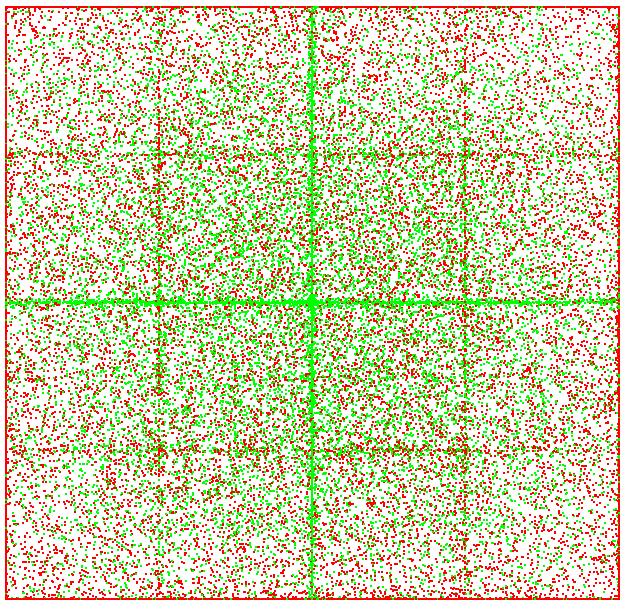
\includegraphics[width=1.0\textwidth, angle=0]{EMERGENT_PATTERN.png}
  	\caption{The emergent pattern used as criteria for qualitative comparison of implementations. Note the big green cross in the center and the smaller red crosses in each sub-sector. World-type is \textit{border} with 100.000 Agents where 25\% are Heroes.}
	\label{fig:EMERGENT_PATTERN}
\end{figure}


\subsection{Problem of RNG}
Have to behave EXACTLY The same: VERY difficult because of differing interfaces e.g. compare java to haskell RNGs.
Solution: create a deterministic RNG generating a number-stream starting from 1 and just counting up. The program should work also in this case, if not, something should be flawed!

Peer told me to implement a RNG-Trace: generate a list of 1000.0000 pre-calculated random-numbers in range of [0..1], store them in a file and read the trace in all implementations. Needs lots of implementation.

\subsection{Run-Time Complexity}
what if the number of agents grows? how does the run-time complexity of the simulation increases? Does it differ from implementation to implementation? The model is O(n) but is this true for the implementation?

\subsection{Simulation-Loops}
There are at least 2 parts to implementing a simulation: 1. implementing the logic of an agent and 2. implementing the iteration/recursion which drives the whole simulation

Classic \\
Yampa \\ TODO: use par to parallelize
Gloss \\
gloss provides means for simple simulation using simulate method. But: are all ABM systems like that?

\subsection{Agent-Representation}
Java: (immutable) Object
Haskell Classic: a struct
Haskell Yampa: a Signal-Function
Gloss: same as haskell classic
Akka: Actors

\subsection{EDSL}
simplify simulation into concise EDSL: distinguish between different kind if sims: continuous/discrete iteration on: fixed set, growing set, shrinking set, dynamic set. 

\section{Adding Spatiality}
When emulating the dynamics of the SIR model using an agent-based approach the question arises what we ultimately gain from doing so when we could have generated the dynamics much quicker and smoother using the SD approach. The difference is that the agent-based approach is a stochastic one and can thus also result in "degenerated" dynamics in which the disease dies out after a few steps or even can't spread from patient zero - in this case ABS is clearly a benefit as it allows to investigate \textit{alternative futures}, something not possible with SD in which the disease will never die out prematurely when there are non-zero infected agents. \\
Another advantage of ABS over SD is that agents can be heterogeneous and make use of spatial- and/or network-information defining the neighbourhood. We can thus simulate the spread of the disease throughout a population which is laid out on a 2D grid or one can investigate spreading of the disease throughout a network of agents where some are vaccinated and others not. We provide already suitable environments to simulate these cases and show an example of spreading the disease on a 2D grid in Figure \ref{fig:sir_spatial}.  

\begin{figure*}
\begin{center}
	\begin{tabular}{c c}
		\begin{subfigure}[b]{0.4\textwidth}
			\centering
			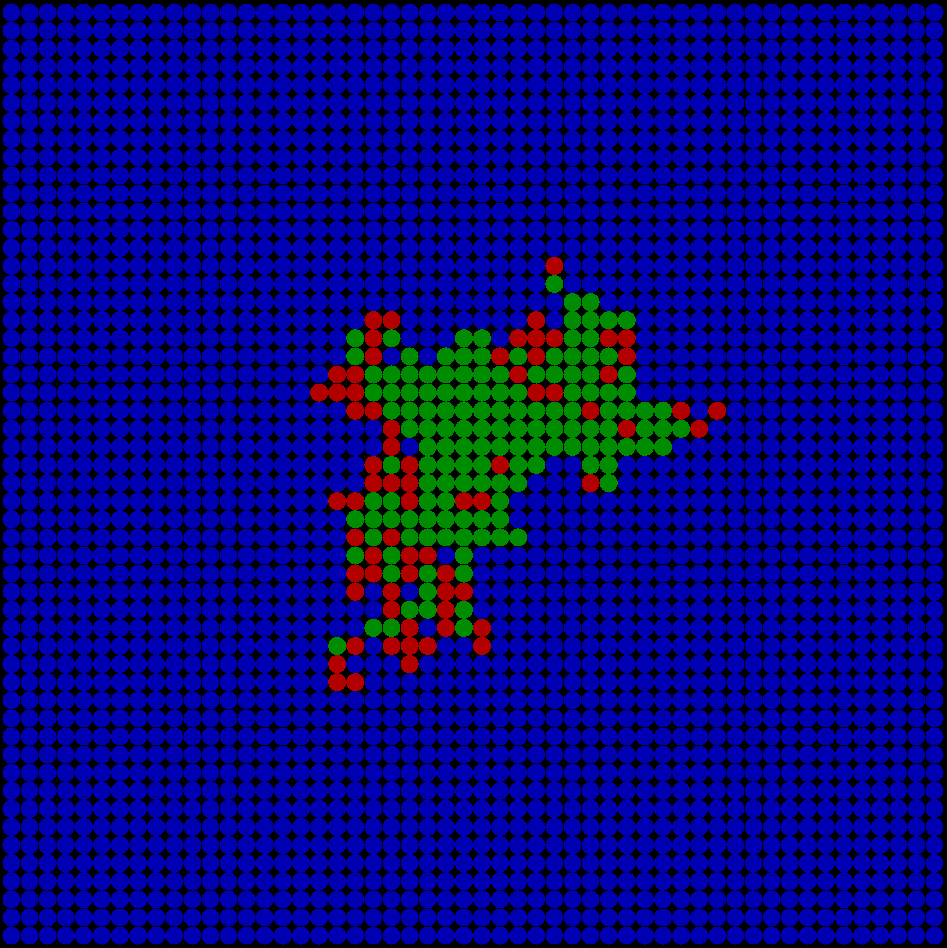
\includegraphics[width=.6\textwidth, angle=0]{./../shared/fig/spatial/SIR_spatial_52x52_92time.png}
			\caption{$t = 92$}
			\label{fig:sir_spatial_92}
		\end{subfigure}

		& 

		\begin{subfigure}[b]{0.4\textwidth}
			\centering
			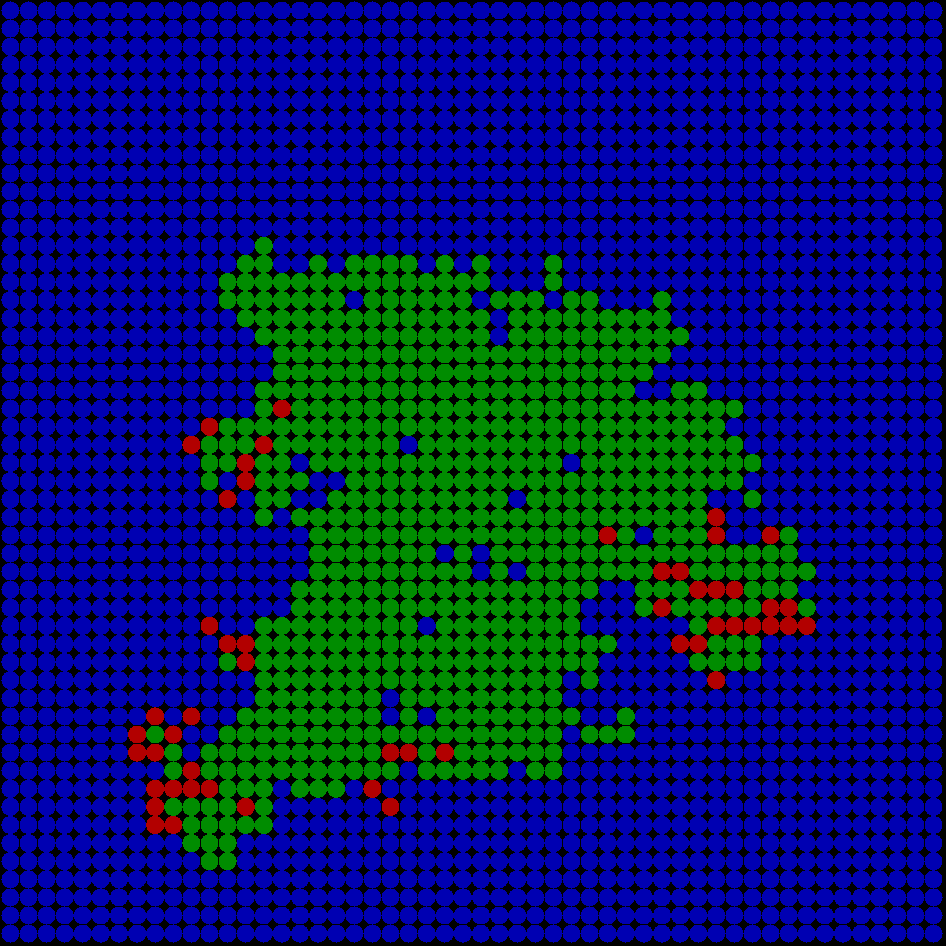
\includegraphics[width=.6\textwidth, angle=0]{./../shared/fig/spatial/SIR_spatial_52x52_200time.png}
			\caption{$t = 200$}
			\label{fig:sir_spatial_200}
		\end{subfigure}

		\\
		
		\begin{subfigure}[b]{0.4\textwidth}
			\centering
			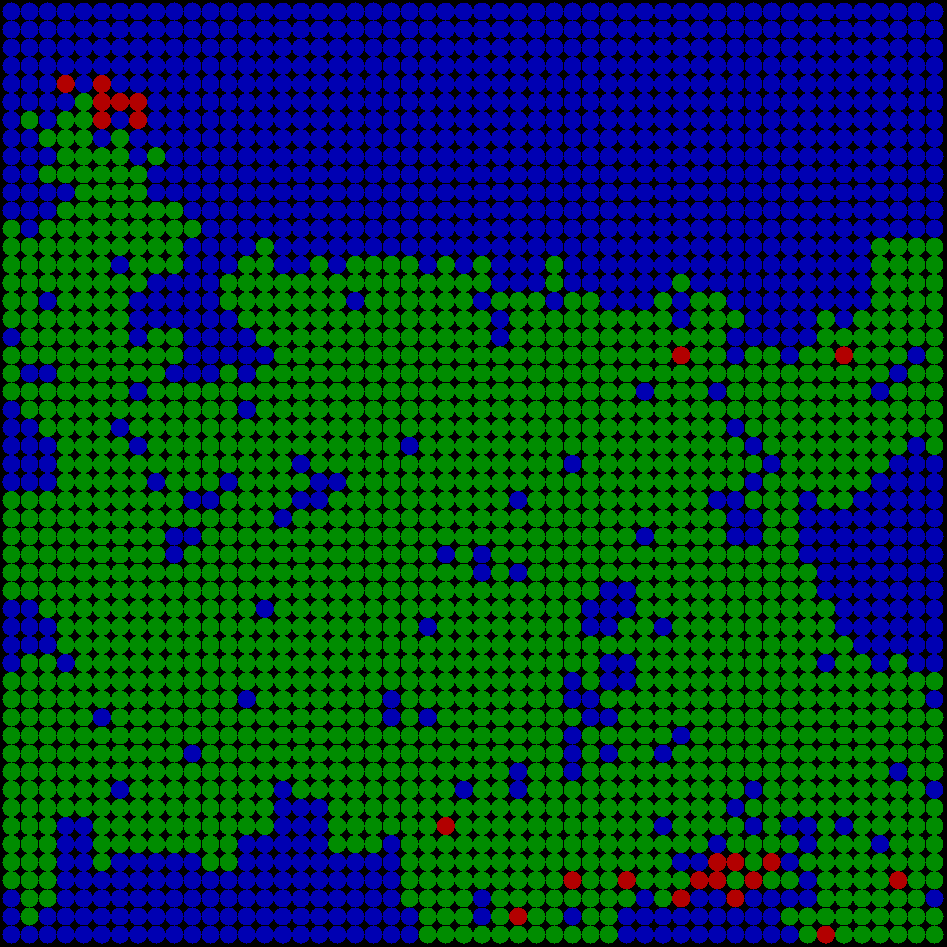
\includegraphics[width=.6\textwidth, angle=0]{./../shared/fig/spatial/SIR_spatial_52x52_440time.png}
			\caption{$t = 440$}
			\label{fig:sir_spatial_440}
		\end{subfigure}
		
		& 
		
		\begin{subfigure}[b]{0.4\textwidth}
			\centering
			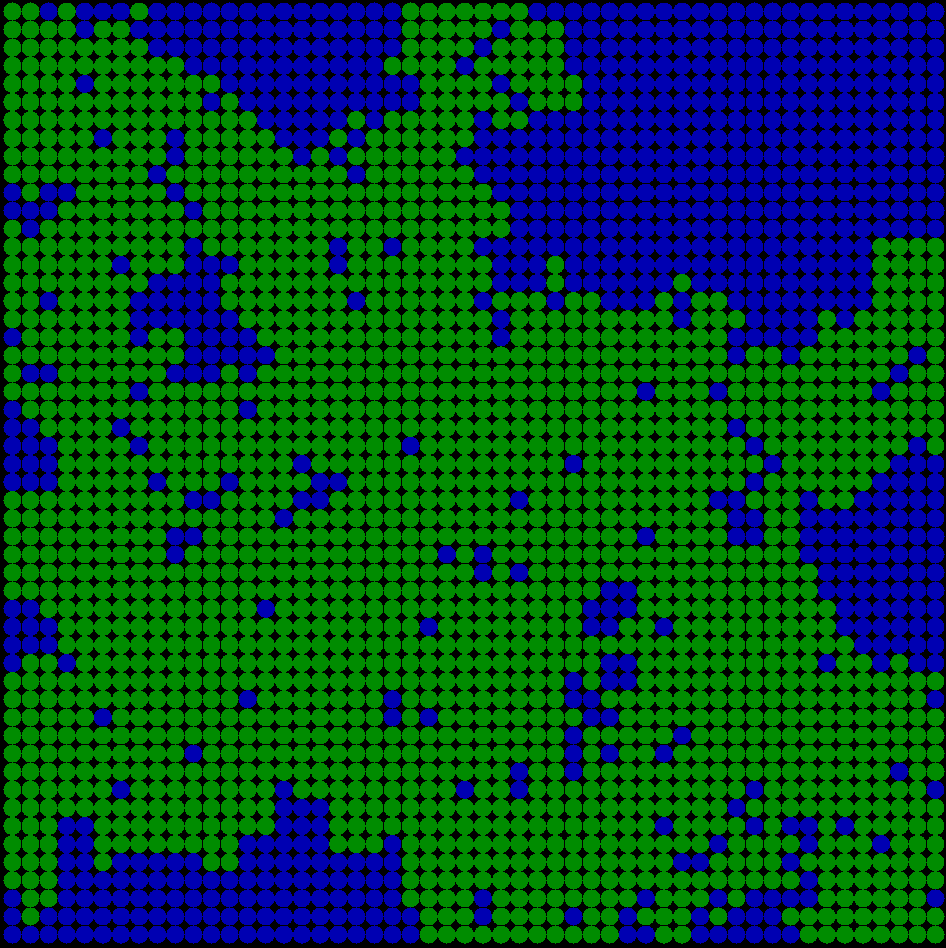
\includegraphics[width=.6\textwidth, angle=0]{./../shared/fig/spatial/SIR_spatial_52x52_873time.png}
			\caption{$t = 873$}
			\label{fig:sir_spatial_873}
		\end{subfigure}
	\end{tabular}
	
	\caption{Simulating SIR on a 52x52 grid with Moore neighbourhood using $\Delta t = 1$. Blue are susceptible, red are infected, green are recovered. The green areas act as protection as infected cannot cross the recovered border: this is particularly visible in the lower right corner of \ref{fig:sir_spatial_440} where the disease has been contained in the blue island and has no means to escape. It may seem that the few remaining infected agents in the top left corner of \ref{fig:sir_spatial_440} will die out soon but still it needs more than the already running simulation time until the disease actually dies out with the last patient recovering at center top of \ref{fig:sir_spatial_873} at $t = 873$. The dynamics of this simulation run can be seen in Figure \ref{fig:sir_spatial_dynamics}.} 
	\label{fig:sir_spatial}
\end{center}
\end{figure*}

\begin{figure}
	\centering
	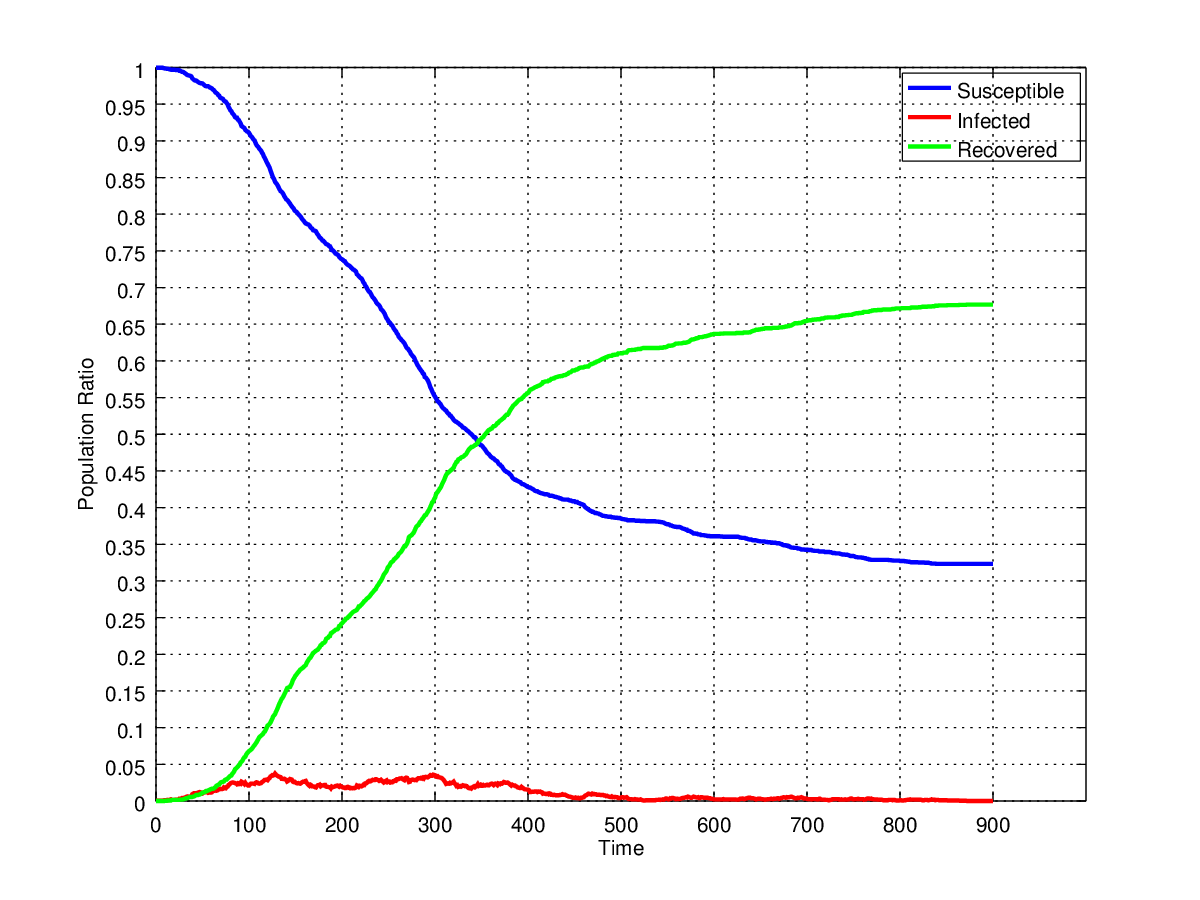
\includegraphics[width=.6\textwidth, angle=0]{./../shared/fig/spatial/SIR_spatial_dynamics_52x52_900time_1dt_parallel.png}
	\caption{Dynamics of the spatial SIR simulation from Figure \ref{fig:sir_spatial}.}
	\label{fig:sir_spatial_dynamics}
\end{figure}

Note that the dynamics of the spatial SIR simulation which are seen in Figure \ref{fig:sir_spatial_dynamics} look very different from the SD dynamics of Figure \ref{fig:sir_sd_dynamics}. This is due to a much more restricted neighbourhood which results in far fewer infected agents at a time and a lower number of recovered agents at the end of the epidemic, meaning that fewer agents got infected overall.

When using a 2D grid or network one needs to set them up in the initialization code so there is a little more work to do there but the implementation of the agents differ just in one single line, which is where the neighbourhood is picked - see line 100 of Appendix \ref{app:abs_code}. Instead of \textit{randomAgentIdMsgSource} one uses either \textit{randomNeighbourNodeMsgSource} in the case of a network or \textit{randomNeighbourCellMsgSource} in case of a 2D grid.

\section{Randomness and Super-Sampling}
TODO: maybe this subsection is unimportant

It is important to note that if we disable super-sampling and run the simulation for a given time \textit{t} but with two different $\Delta t$ we would end up with two different results, even if the $\Delta t$ are small enough to sample the time-dependent functions sufficiently. Also if we use super-sampling with $\Delta t = 1.0$ and create the exact same number of samples as when using no super-sampling but smaller $\Delta t$, then we also end up with different results.
The reason for this behaviour is that most of the time-dependent functions ultimately build upon drawing from random-distributions. With different $\Delta t$ we are generating a different number of random-samples, which would result in different random-number sequences which in turn ultimately leads to slightly different dynamics. When generating a plot of the dynamics this is not as visible, also this is the reason why one generates multiple replications, but this behaviour becomes strikingly apparent when simulating the SIR model on a 2D grid as can be seen in Figure \ref{fig:sir_abs_timeDeltas_randomness}.

\begin{figure*}
\begin{center}
	\begin{tabular}{c c}
		\begin{subfigure}[b]{0.4\textwidth}
			\centering
			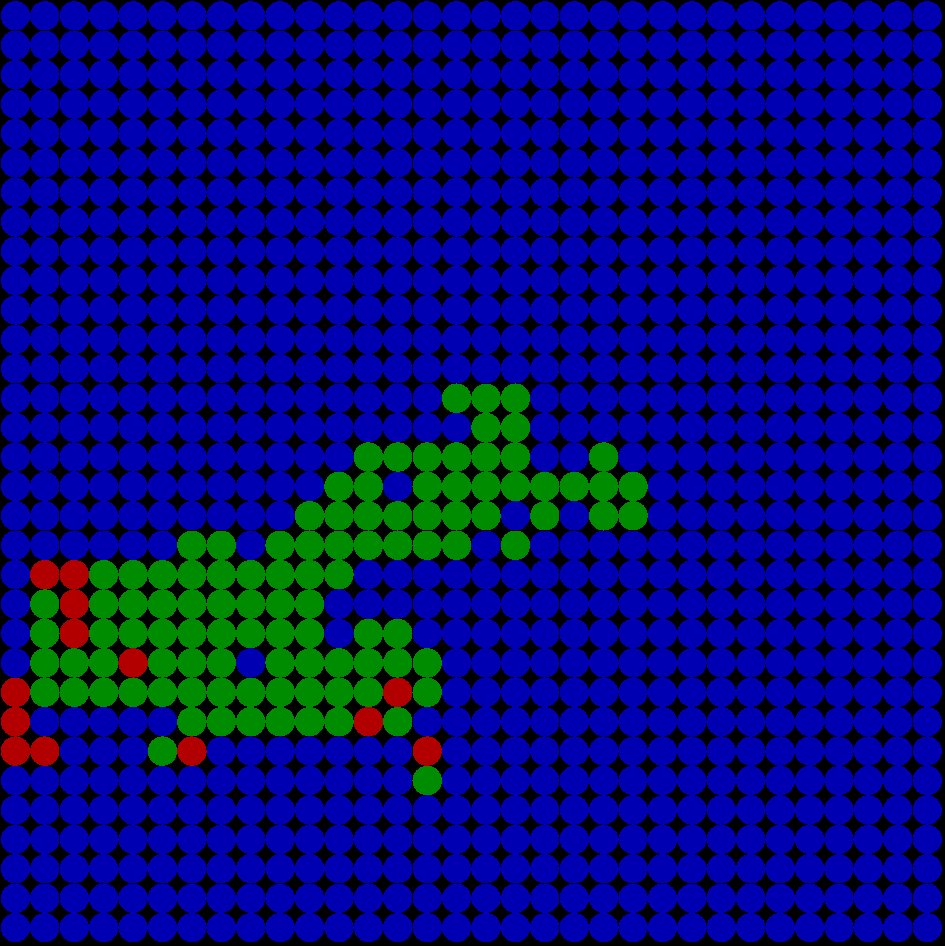
\includegraphics[width=.7\textwidth, angle=0]{./shared/fig/randomness/SIR_32x32_200time_01delta_noSS.png}
			\caption{$\Delta t = 0.1$, no super-sampling}
			\label{fig:sir_abs_timeDeltas_randomness_dt01}
		\end{subfigure}
	
		& 
		
		\begin{subfigure}[b]{0.4\textwidth}
			\centering
			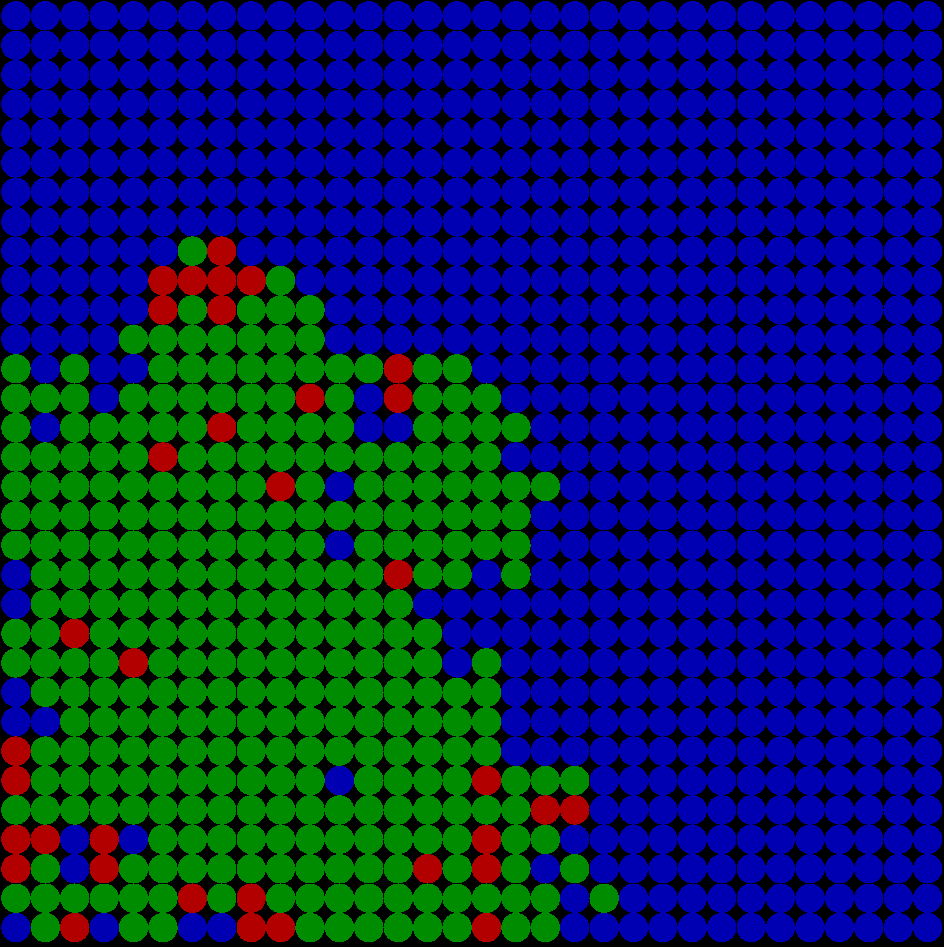
\includegraphics[width=.7\textwidth, angle=0]{./shared/fig/randomness/SIR_32x32_200time_001delta_noSS.png}
			\caption{$\Delta t = 0.01$, no super-sampling}
			\label{fig:sir_abs_timeDeltas_randomness_dt001}
		\end{subfigure}
		
		\\

		\begin{subfigure}[b]{0.4\textwidth}
			\centering
			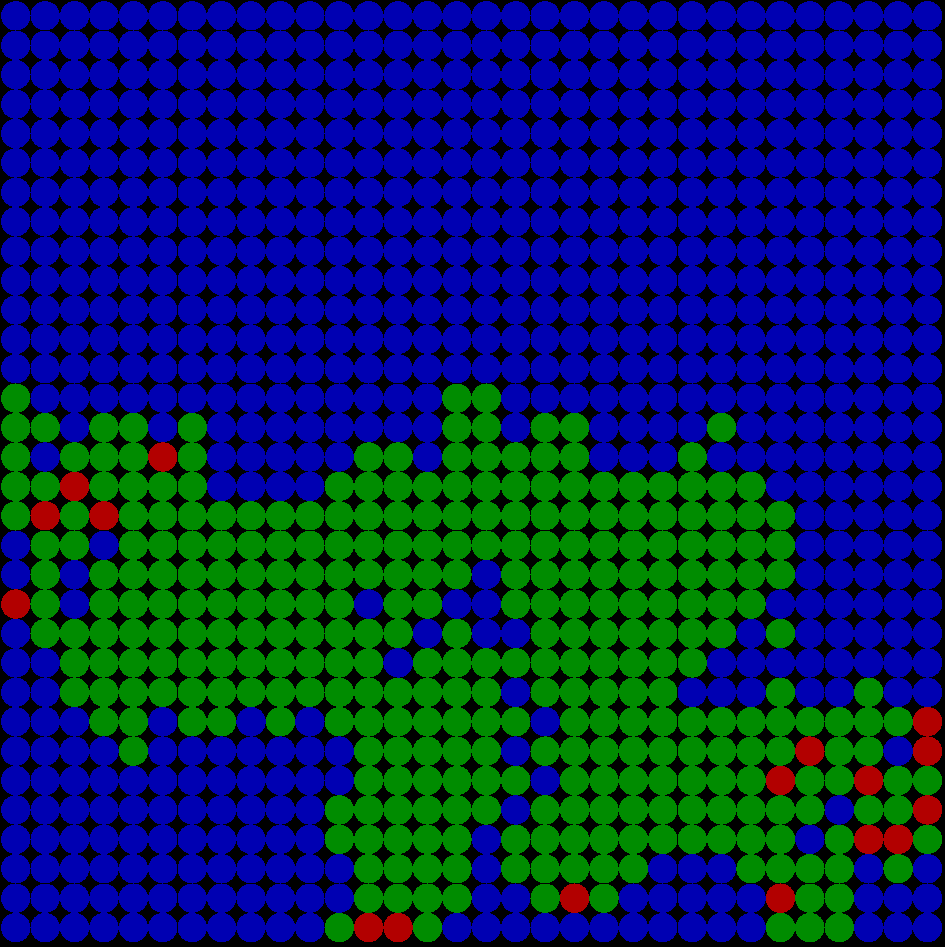
\includegraphics[width=.7\textwidth, angle=0]{./shared/fig/randomness/SIR_32x32_200time_10delta_ss10.png}
			\caption{$\Delta t = 1.0$ with 10 super-samples}
			\label{fig:sir_abs_timeDeltas_randomness_dt10_ss10}
		\end{subfigure}
		
		&
		
		\begin{subfigure}[b]{0.4\textwidth}
			\centering
			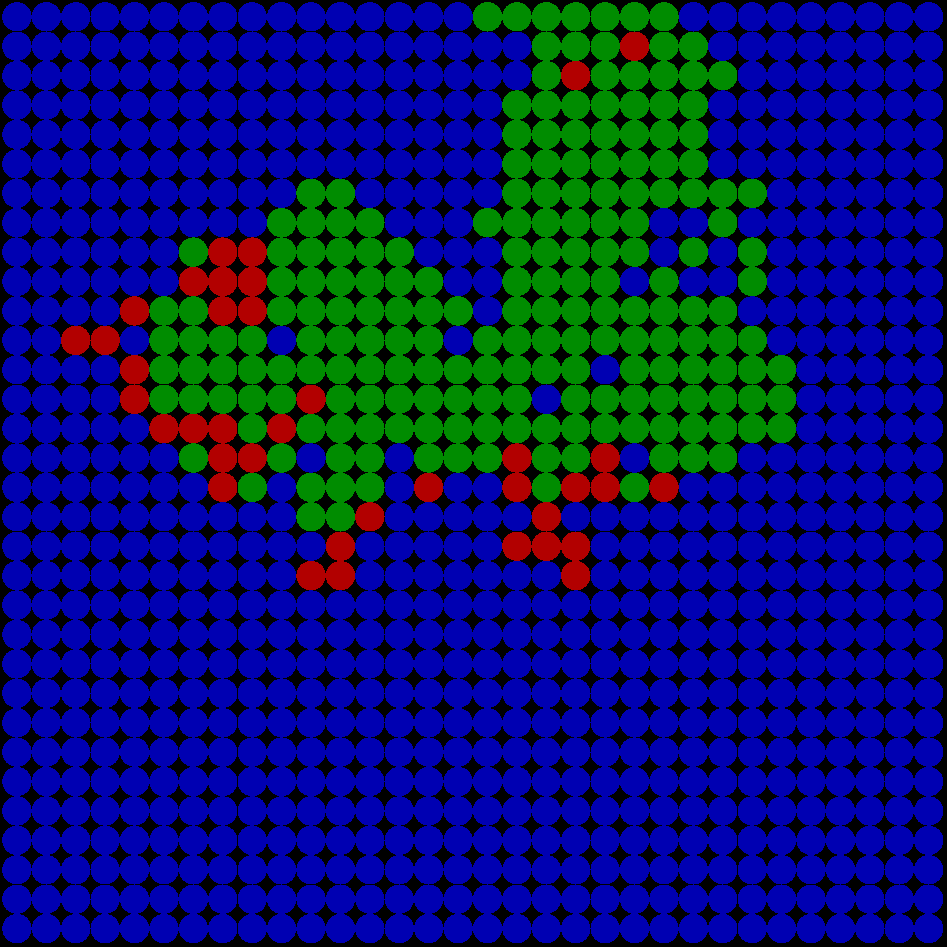
\includegraphics[width=.7\textwidth, angle=0]{./shared/fig/randomness/SIR_32x32_200time_10delta_ss100.png}
			\caption{$\Delta t = 1.0$ with 100 super-samples}
			\label{fig:sir_abs_timeDeltas_randomness_dt10_ss100}
		\end{subfigure}
	\end{tabular}
	
	\caption{Comparing results on 32x32 grid after $t = 200$ but with different $\Delta t$ and different number of super-samples.}
	\label{fig:sir_abs_timeDeltas_randomness}
\end{center}
\end{figure*}

\section{Agents as Signals}
Due to the underlying nature and motivation of FRP and Yampa, agents can be seen as signals which are generated and consumed by a signal-function which is the behaviour of an agent.  If an agent does not change, the output-signal should be constant amd if the agent changes e.g. by sending a message, changing its state,... the output-signal should change as well. A dead agent then should have no signal at all.
The question is if the agents of our agent-based SIR implementation are true signals: do the dynamics stay constant when we sample the system with $\Delta t = 0$? We hypothesize that our agents are true signals, thus they should not change when time does not change because they are completely time-dependent and rely completely on time-semantics. When actually running the simulation with $\Delta t = 0$ one gets the results as seen in Figure \ref{fig:sir_abs_zero_dt}.

\begin{figure*}
\begin{center}
	\begin{tabular}{c c}
		\begin{subfigure}[b]{0.5\textwidth}
			\centering
			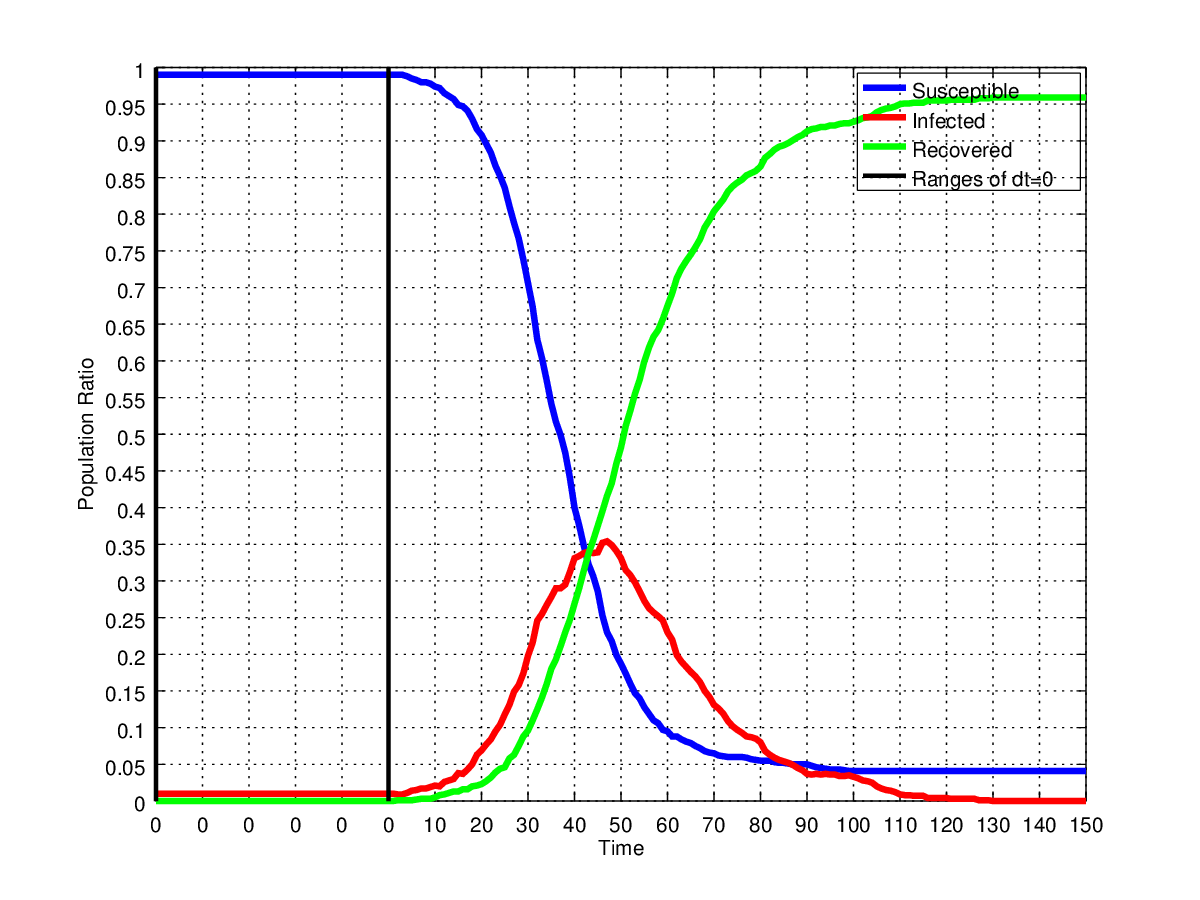
\includegraphics[width=.8\textwidth, angle=0]{./../shared/fig/dtzero/SIR_ABS_zeroDt_start.png}
			\caption{$\Delta t = 0$ from step 0 to 50.}
			\label{fig:sd_plot_10dt}
		\end{subfigure}
	
		& 
		
		\begin{subfigure}[b]{0.5\textwidth}
			\centering
			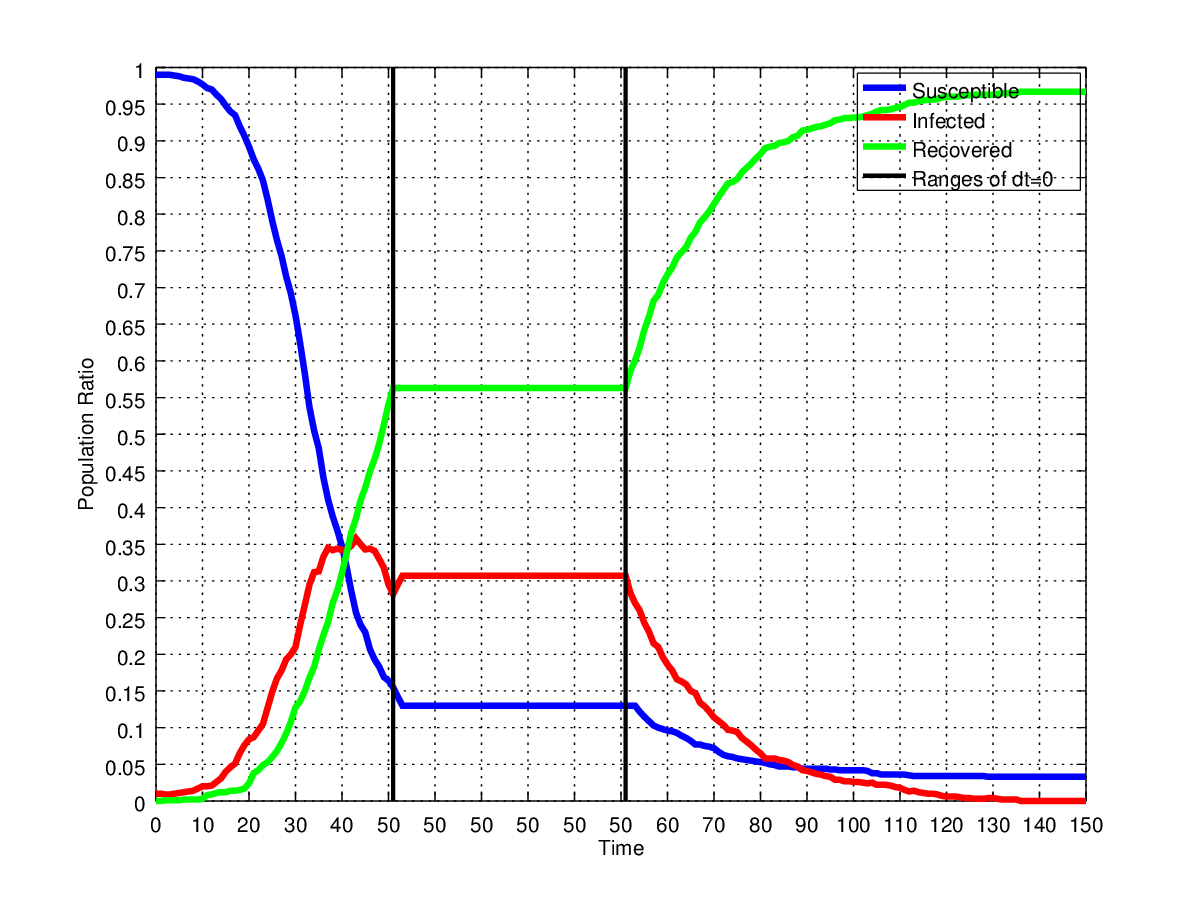
\includegraphics[width=.8\textwidth, angle=0]{./../shared/fig/dtzero/SIR_ABS_zeroDt_mid.png}
			\caption{$\Delta t = 0$ from step 51 to 101.}
			\label{fig:sd_plot_0.01dt}
		\end{subfigure}
	\end{tabular}
	
	\caption{Dynamics of agent-based SIR implementation of 1,000 agents running with $\Delta t = 1$ with ranges of $\Delta t = 0$ marked with two vertical black lines.}
	\label{fig:sir_abs_zero_dt}
\end{center}
\end{figure*}

As can be seen  the dynamics are becoming constant \textit{but} with a minor delay: infected increases a bit while susceptible decreases as can be seen in Figure \ref{fig:sir_abs_zero_dt_zoom}. This is due to the delay of message delivery which takes one $\Delta t$, independent of its value - messages are also delivered when $\Delta t = 0$. Only message-generating functions, which depend on non-zero $\Delta t$ to generate messages, will then stop generating messages. Reactive functions which act on incoming messages can still create change as they do not rely on time-semantics but just on the discrete event of a message arrival - which is the case in the transition from susceptible to infected.

\begin{figure}
	\centering
	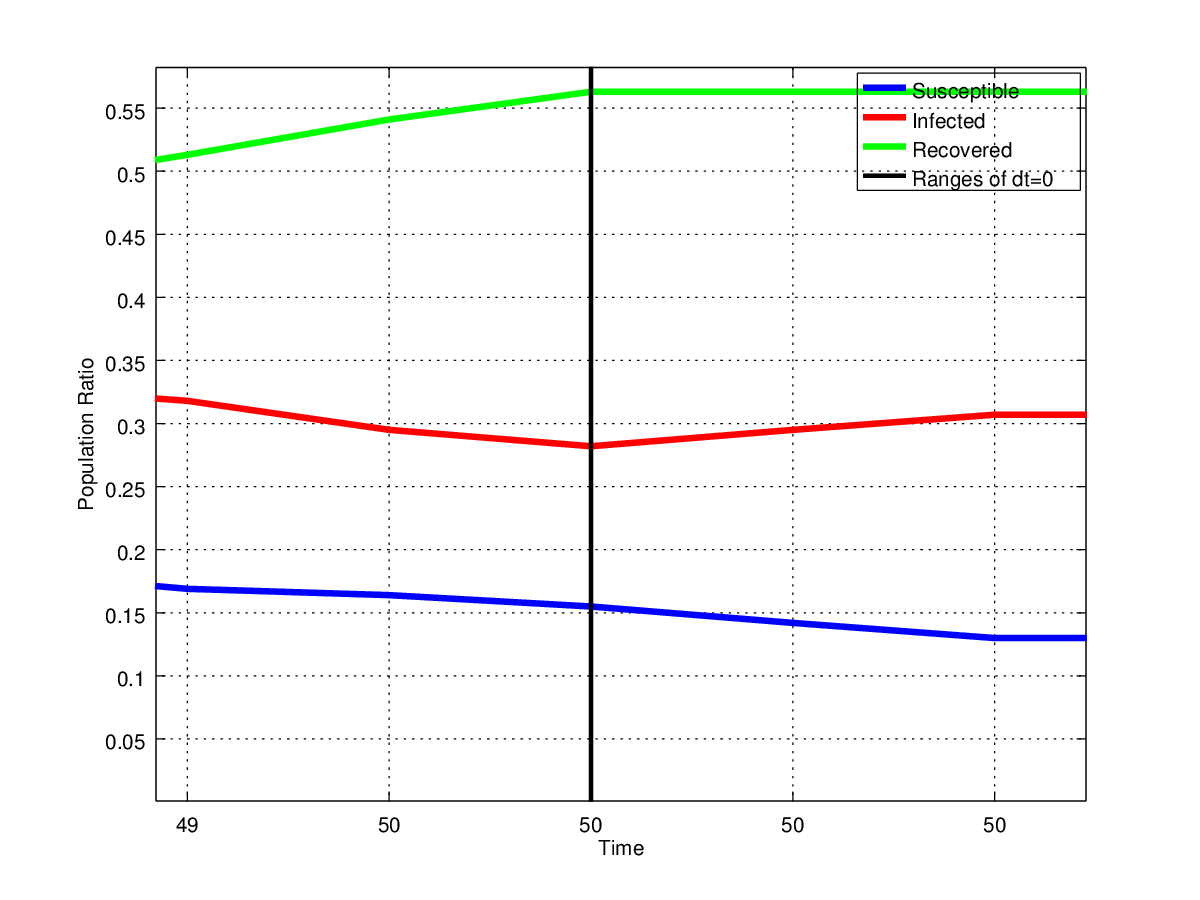
\includegraphics[width=.4\textwidth, angle=0]{./../shared/fig/dtzero/SIR_ABS_zeroDt_mid_zoom.png}
	\caption{Zoom-in to step 51, marked with the black line from where on $\Delta t = 0$ for the next 50 steps. The recovered ratio stays constant but a few agents get infected even \textit{after} having switched to $\Delta t = 0$ which happens due to the message delivery lag. After all messages have been delivered, the signal stays constant until non-zero $\Delta t$ are turned on again.}
	\label{fig:sir_abs_zero_dt_zoom}
\end{figure}

Note that agents of models with no time-semantics won't exhibit this behaviour - the dynamics will change even in case of $\Delta t = 0$ as agents act on every update and don't care about $\Delta t$ and just assume that every update occurs after $\Delta t$ independent of the actual value of it. We implemented the function \textit{doRepeatedlyEvery} which allows to transform a time-agnostic agent-behaviour into one. It is built on Yampas \textit{repeatedly} function and has the following signature:

\begin{minted}[fontsize=\footnotesize]{haskell}
doRepeatedlyEvery :: Time -> AgentBehaviour -> AgentBehaviour
\end{minted}

This function takes a time interval and an agent behaviour signal-function and returns a new agent behaviour signal-function which runs the argument signal-function every time-interval. Note that this function is subject to sampling issues. When the time-interval is very small one needs to run the simulation with a $\Delta t \leq Time$ otherwise the dynamics would show delayed activation of the agent behaviour.

\section{Discussion}
Although there are similarities to the work of \cite{botta_time_2010} (the use of messages and the problem of when to advance time in models with arbitrary number synchronised agent-interactions), we approach our agents differently. First in our approach an agent is only a single MSF and thus can not be directly queried for its internal state / its id or outgoing messages, instead of taking a list of messages, our agents take a single event/message and can produce an arbitrary number of outgoing messages together with an observable state - note that this would allow to query the agent for its id and its state as well by simply sending a corresponding message to the agents MSF and requiring the agent to implement message handling for it. Also the state of our agents is \textit{completely} localised and there is no means of accessing the state from outside the agent, they are thus "fully encapsulated agents" \cite{botta_time_2010}. Note that the authors of \cite{botta_time_2010} define their agents with a polymorphic agent-state type \textit{s}, which implies that without knowledge of the specific type of \textit{s} there would be no way of accessing the state, rendering it in fact also fully encapsulated. The problem of advancing time in our approach is solved not exactly the same but conceptually it is the same: after sending a tick message to each agent (in random order), we process all agents until they are idle: there are no more enqueued messages / events in the queue.

our eventdriven approach makes heavy use of 2 state monads, thus one might ask what the benefits are, after all we seem to fall back into stateful, imperative style programming. we agree that our approach is just one way of implementing abs in fp but we think we have come a long way thus making our approach quite valuable even if there might be other approaches like shallow EDSLs. on the other hand even our stateful programming is highly restricted to only those 2 local datatypes which makes it much more manageable than unrestricted data mutation

quote carmack (\url{http://www.gamasutra.com/view/news/169296/Indepth_Functional_programming_in_C.php}): the main difficulty as a developer in software programming is to keep track of the states a program can be in and reason about them and their Validity

TODO: report LoC and compare it with other implementations we found on the internet

\section{Related Research}
Already noted in the Introduction, \cite{huberman_evolutionary_1993} where the first to discuss the differences update-strategies can make and introduced the terms of synchronous and asynchronous updates. They define to be synchronous as agents being updated in unison and asynchronous where one agent is updated and the others are held constant.

\medskip

\cite{a_framework_2008} give an approach for ABS on GPUs which is a very different approach to updating and iterating agents in ABS. They discuss execution order at length, highlight the problem of inducing a specific execution-order in a model which is problematic for parallel execution and give solutions how to circumvent these shortcomings. Although we haven't mapped our ideas to GPUs we explicitly include an approach for data-parallelism which, we hypothesize, can be utilized to roughly map their approach onto our terminology. 
	
\medskip
	
\cite{botta_time_2010} sketch a minimal ABS implementation in Haskell which is very similar in the basic structure of ours. This proves that our approach seems to be a very natural one to apply to Haskell. Their focus is primarily on economic simulations and instead of iterating a simulation with a global time, their focus is on how to synchronize agents which have internal, local transition times. Although their work uses Haskell as well, our focus is very different from theirs and approaches ABS in a more general and comprehensive way.

\medskip

\cite{dawson_opening_2014} describe basic inner workings of ABS environments and compare their implementation in C++ to the existing ABS environment AnyLogic which is programmed in Java. They explicitly mention asynchronous and synchronous time-models and compare them in theory but unfortunately couldn't report the results of asynchronous updates due to limited space. They interpret asynchronous time-models to be the ones in which an agent acts at random time intervals and synchronous time-models where agents are updated all in same time intervals.

\medskip

\cite{yuxuan_agent-based_2016} presents in his Master-Thesis a comprehensive discussion on how to implement an ABS for state-charts in Java and also mentions synchronous and asynchronous time-models. He identifies the asynchronous time-model to be one in which updates are triggered by the exchange of messages and the synchronous ones which trigger changes immediately without the indirection of messages.

\medskip

We observe that there seems to be a variety of meanings attributed to the terminology of asynchronous and synchronous updates but the very semantic and technical details are unclear and not described very precisely. In the next section we will address this issue by presenting the basic background and propose properties for a new terminology from which we can derive common update-strategies.

\section{Conclusion and further research}

So far we only looked at recursive simulation in a simulation with a strictly sequential update-strategy where agents are updated in sequence after each other as defined in TODO: cite my Art-Of-Iteration Paper. We leave the question of how Meta-ABS would apply to the parallel update-strategy and whether it is reasonable to extend it to that strategy or not for further research.

Research Questions
\begin{enumerate}
	\item How does deep regression influence the dynamics of a system? Hypothesis: TODO
	\item How do the dynamics of a system change when using perfect information or learning local information? Hypothesis: TODO
	\item Is a hidden markov model suitable for the local learning? Hypothesis: TODO
	\item How can MetaABS best be implemented? Hypothesis: implementing a MetaABS EDSL in a pure functional language like Haskell, should be best suited due to its inherent recursive, declarative nature, which should allow a direct mapping of features of this paradigm to the specification of the meta-model
\end{enumerate}

Problems
\begin{itemize}
	\item Definition of a recursive, declarative description of the Model.
	\item Perfect information about other agents is not realistic and runs counter to agent-based simulation (especially in social sciences) thus an Agent needs to be able to have local, noisy representations of the other agents.
	\item Local representation of other agents could be captured by Hidden Markov Models: observe what other agents do but have hidden interpretation of their internal state - these internal state-representations can be different between the local and the global version whereas the agent learns to represent the global version as best as possible locally.
	\item Infinite regress is theoretically possible but not on computers, we need to terminate at some point
\end{itemize}

\section*{Acknowledgments}
The authors would like to thank I. Perez, H. Nilsson, J. Greensmith, T. Schwarz and H. Vollbrecht for constructive comments and valuable discussions.

\bibliographystyle{../../../templates/IEEEtran/bibtex/IEEEtran}
\bibliography{../../../../references/phdReferences.bib}

\appendices

\newpage
\section{Full code of the agent-based SIR implementation}
\label{app:abs_code}

\begin{minted}[fontsize=\footnotesize, linenos]{haskell}
data SIRState = Susceptible | Infected | Recovered deriving (Eq)
data SIRMsg = Contact SIRState deriving (Eq)

type SIRAgentState = SIRState

type SIREnvironment = [AgentId]

type SIRAgentDef = AgentDef SIRAgentState SIRMsg SIREnvironment
type SIRAgentBehaviour = AgentBehaviour SIRAgentState SIRMsg SIREnvironment
type SIRAgentBehaviourReadEnv = ReactiveBehaviourReadEnv SIRAgentState SIRMsg SIREnvironment
type SIRAgentBehaviourIgnoreEnv = ReactiveBehaviourIgnoreEnv SIRAgentState SIRMsg SIREnvironment
type SIRAgentIn = AgentIn SIRAgentState SIRMsg SIREnvironment
type SIRAgentOut = AgentOut SIRAgentState SIRMsg SIREnvironment
type SIRAgentObservable = AgentObservable SIRAgentState

type SIREventSource = EventSource SIRAgentState SIRMsg SIREnvironment

-------------------------------------------------------------------------------
infectivity :: Double
infectivity = 0.05

contactRate :: Double
contactRate = 5

illnessDuration :: Double
illnessDuration = 15

contactSS :: Int
contactSS = 20

illnessTimeoutSS :: Int
illnessTimeoutSS = 2

-------------------------------------------------------------------------------
createSIRNumInfected :: Int -> Int -> IO ([SIRAgentDef], SIREnvironment)
createSIRNumInfected agentCount numInfected = do
    let agentIds = [0 .. (agentCount-1)]
    let infectedIds = take numInfected agentIds
    let susceptibleIds = drop numInfected agentIds

    adefsSusceptible <- mapM (sirAgent Susceptible) susceptibleIds
    adefsInfected <- mapM (sirAgent Infected) infectedIds

    return (adefsSusceptible ++ adefsInfected, agentIds)

sirAgent :: SIRState -> AgentId -> IO SIRAgentDef
sirAgent initS aid = do
    rng <- newStdGen
    let beh = sirAgentBehaviour rng initS
    let adef = AgentDef { 
          adId = aid
        , adState = initS
        , adBeh = beh
        , adInitMessages = NoEvent
        , adConversation = Nothing
        , adRng = rng 
        }

    return adef
   
-------------------------------------------------------------------------------
-- UTILITIES
gotInfected :: SIRAgentIn -> Rand StdGen Bool
gotInfected ain = onMessageM gotInfectedAux ain False
  where
    gotInfectedAux :: Bool -> AgentMessage SIRMsg -> Rand StdGen Bool
    gotInfectedAux False (_, Contact Infected) = randomBoolM infectivity
    gotInfectedAux x _ = return x



respondToContactWith :: SIRState -> SIRAgentIn -> SIRAgentOut -> SIRAgentOut
respondToContactWith state ain ao = onMessage respondToContactWithAux ain ao
  where
    respondToContactWithAux :: AgentMessage SIRMsg -> SIRAgentOut -> SIRAgentOut
    respondToContactWithAux (senderId, Contact _) ao = sendMessage (senderId, Contact state) ao

-- SUSCEPTIBLE
sirAgentSuceptible :: RandomGen g => g -> SIRAgentBehaviour
sirAgentSuceptible g = 
	transitionOnEvent 
		sirAgentInfectedEvent 
		(readEnv $ sirAgentSusceptibleBehaviour g) 
		(sirAgentInfected g)

sirAgentInfectedEvent :: SIREventSource
sirAgentInfectedEvent = proc (ain, ao) -> do
    let (isInfected, ao') = agentRandom (gotInfected ain) ao 
    infectionEvent <- edge -< isInfected
    returnA -< (ao', infectionEvent)

sirAgentSusceptibleBehaviour :: RandomGen g => g -> SIRAgentBehaviourReadEnv
sirAgentSusceptibleBehaviour g = proc (ain, e) -> do
    ao' <- doOnce (setAgentState Susceptible) -< agentOutFromIn ain
    returnA -< sendMessageOccasionallySrcSS 
    			g
    			(1 / contactRate)
    			contactSS
    			(randomAgentIdMsgSource (Contact Susceptible) True) -< (ao', e)

-- INFECTED
sirAgentInfected :: RandomGen g => g -> SIRAgentBehaviour
sirAgentInfected g = 
	transitionAfterExpSS 
		g 
		illnessDuration 
		illnessTimeoutSS 
		(ignoreEnv $ sirAgentInfectedBehaviour g) 
		sirAgentRecovered

sirAgentInfectedBehaviour :: RandomGen g => g -> SIRAgentBehaviourIgnoreEnv
sirAgentInfectedBehaviour g = proc ain -> do
    ao' <- doOnce (setAgentState Infected) -< agentOutFromIn ain
    returnA -< respondToContactWith Infected ain ao'

-- RECOVERED
sirAgentRecovered :: SIRAgentBehaviour
sirAgentRecovered = doOnceR $ setAgentStateR Recovered

-- INITIAL CASES
sirAgentBehaviour :: RandomGen g => g -> SIRState -> SIRAgentBehaviour
sirAgentBehaviour g Susceptible = sirAgentSuceptible g
sirAgentBehaviour g Infected = sirAgentInfected g
sirAgentBehaviour _ Recovered = sirAgentRecovered

-------------------------------------------------------------------------------
runSIR :: IO ()
runSIR = do
    -- parallel strategy, no updating/folding of environment, no shuffling, rng-seed of 42
    params <- initSimulation Parallel Nothing Nothing False (Just 42)
    (initAdefs, initEnv) <- createSIRNumInfected agentCount numInfected
    let dynamics = simulateAggregateTime initAdefs initEnv params dt t aggregate
    print dynamics
	
aggregate :: (Time, [SIRAgentObservable], SIREnvironment) -> (Time, Double, Double, Double)
aggregate (t, aobs, _) = (t, susceptibleCount, infectedCount, recoveredCount)
  where
    susceptibleCount = fromIntegral $ length $ filter ((Susceptible==) . snd) aobs
    infectedCount = fromIntegral $ length $ filter ((Infected==) . snd) aobs
    recoveredCount = fromIntegral $ length $ filter ((Recovered==) . snd) aobs
\end{minted}

\end{document}